	%%%Architettura alto livello%%%
\section{Architettura ad alto livello}
Nella seguente sezione verr\`{a} illustrata l'architettura ad alto livello del sistema sviluppato, 
escludendo i dettagli implementativi e legati al linguaggio. Viene fornito un diagramma delle componenti per fornire un'idea
generale.\\
\begin{center}
\begin{figure}[h!]
	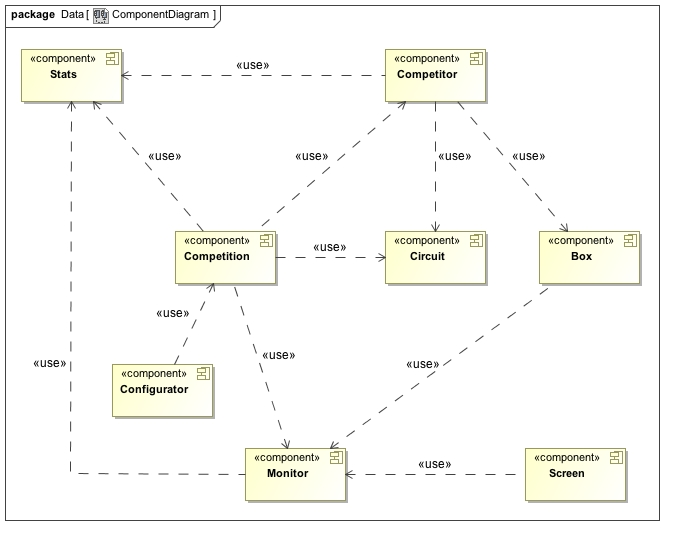
\includegraphics[scale=0.50]{img/ComponentDiagram.jpg}
	\caption{Diagramma delle componenti}
\end{figure}
\end{center}
% Componenti del sistema
\subsection{Componenti di sistema}
Le principali componenti del sistema sono:
\subsubsection{Competition}
La \emph{Competition} \`{e} l'unit\`{a} atta ad orchestrare l'avvio e la conclusione della corsa. Tale componente, dunque, \`{e} stata concepita per 
offrire le seguenti funzionalit\`{a}:
\begin{itemize}
\item Configurazione parametri di gara:
	\begin{itemize}
		\item numero di giri;
		\item numero di concorrenti;
		\item circuito;
	\end{itemize}
\item Gestione della sessione di iscrizione e accettazione concorrenti (configurati a livello della componente \emph{Box})
\item Avvio delle componenti necessarie al monitoraggio della gara (quali ad esempio \emph{Monitor})
\item Avvio controllato della competizione vera e propria nel momento in cui tutti i prerequisiti di inizio sono soddisfatti, ovvero:
\begin{itemize}
\item la competizione \`{e} stata configurata correttamente;
\item le componenti di controllo e gestione della competizione sono attive e in attesa di comandi;
\item i concorrenti sono stati correttamente registrati alla competizione e in attesa di partire;
\end{itemize}
\end{itemize}
\subsubsection{Competitor}
\label{competitor}
Il \emph{Competitor} \`{e} l'entit\`{a} pensata a svolgere la gara. \`{E} caratterizzato dalle seguenti sotto-componenti:
\begin{itemize}
\item \textbf{Auto}, ovvero tutte le caratteristiche fisiche legate all'auto:
	\begin{itemize}
		\item motore;
		\item capacit\`{a} del serbatoio;
		\item massima accelerazione;
		\item massima velocit\`{a};
		\item gomme montate;
		\item livello usura gomme;
		\item livello della benzina nel serbatoio;
	\end{itemize}
\item \textbf{Pilota}, cio\`{e} le informazioni che descrivono pi\`{u} dettagliatamente il concorrente in gara:
	\begin{itemize}
		\item nome e cognome pilota;
		\item nome scuderia
	\end{itemize}
\item \textbf{Strategia}, ovvero la strategia che sta adottando il pilota, suggerita dai box e dinamica nel corso della gara:
	\begin{itemize}
		\item stile di guida, variabile tra conservativo, normale, aggressivo, a seconda dello stato della macchina e delle
			previsioni fatte dai box
		\item numero di lap prima del pit stop
		\item addizionalmente, quando viene fatto un pit stop, la strategia determina anche
		 	la quantit\`{a} di benzina da avere nel serbatoio dopo lo stop e il tempo impiegato per il pit stop (le gomme si assume vengano
		 	cambiate ad ogni pitstop).
	\end{itemize}
\end{itemize}
Tutte queste informazioni insieme creano quello che viene definito il concorrente di gara. 
Tali informazioni verranno poi usate nel corso della gara per:
	\begin{itemize}
		\item scegliere al momento giusto la miglior traiettoria da seguire, in base alle sue caratteristiche (lunghezza, angolo ..)
		 e in base alla presenza o meno di altri concorrenti;
		\item fornire costantemente aggiornamenti sul suo stato (tramite una parte del modulo \emph{Stats}, informando il computer di bordo
			riguardo a:
			\begin{itemize}
				\item livello di usura gomme;
				\item livello di benzina;
				\item checkpoint attraversato con tempo di arrivo;
				\item insieme al checkpoint verranno aggiornate le informazioni relative a settore e lap;
				\item velocit\`{a} massima raggiunta.
			\end{itemize}
		\item contattare ad ogni giro il box per ottenere una strategia aggiornata;
		\item se suggerito dai box, effettuare un pitstop;
		\item ritirarsi dalla gara una volta che le condizioni dell'auto non permettano di poter correre ulteriormente;
		\item banalmente, continuare a correre fino alla fine delle lap prestabilite, dopodich\`{e} fermarsi.
	\end{itemize}
\subsubsection{Circuit}
Il circuito \`{e} una risorsa finalizzata ad offrire il piano su cui svolgere la competizione. \`{E} condivisa fra tutti i concorrenti in gara e
offre un insieme di funzionalit\`{a} per poter conoscere le caratteristiche dei vari tratti della pista (compresi i concorrenti presenti
al momento dell'attraversamento). \`{E} composto dalle seguenti sotto-componenti:
\begin{itemize}
\item \textbf{Checkpoint}:
i \emph{Checkpoint} rappresentano punti di arrivo intermedi del circuito. Come degli intervalli da 1 secondo possono discretizzare 1 minuto,
cos\`{i} i \emph{Checkpoint} discretizzano il circuito. Ogni \emph{Checkpoint} introduce un tratto della pista potenzialmente diverso da quello precedente.
Per esempio, il $\emph{Checkpoint}_n$ potrebbe essere il punto di entrata di un tratto della pista accessibile ad un numero massimo di 4 concorrenti insieme,
mentre il successivo $\emph{Checkpoint}_{n+1}$ potrebbe esporre un tratto pi\`{u} stretto e quindi accessibile solo a 2 concorrenti. Schematizzando, 
il \emph{Checkpoint} \`{e} caratterizzato da:
\begin{itemize}
\item \textbf{molteplicit\`{a}}: ovvero il numero di concorrenti che possono trovarsi contemporaneamente nel tratto a seguire;
\item \textbf{posizione nella pista}: un \emph{Checkpoint} pu\`{u} essere il traguardo, l'inizio del settore, la fine di un settore, all'uscita dei box, l'entrata
					per i box, i box oppure un punto intermedio fra altri due \emph{Checkpoint};
\item \textbf{tempi di arrivo}: ogni \emph{Checkpoint} tiene traccia dell'istante in cui un concorrente ci \`{e} passato sopra.
\end{itemize}
\item \textbf{Path}: rappresenta una delle possibili traiettorie da usare per andare da un \emph{Checkpoint} a quello successivo. La traiettoria presenta
	un numero di \emph{Path} uguale alla molteplicit\`{a} del \emph{Checkpoint} che la precede. Ogni \emph{Path} \`{e} descritto da:
	\begin{itemize}
		\item lunghezza
		\item angolo
		\item grip, ovvero l'aderenza sul tratto
	\end{itemize}
Normalmente i path appartenenti allo stesso tratto differiscono di poco.
\item \textbf{Iteratore}: l'unit\`{a} permette di sapere la struttura della pista. Si suppone venga usata per sapere quale \emph{Checkpoint} ne segue un altro,
	oppure per sapere dove sia il \emph{Checkpoint} di inizio box. 
\end{itemize}
\subsubsection{Stats}
Questa componente mantiene la storia della gara e offre un insieme di funzionalit\`{a} che permettono di elaborare tali dati per offrirne differenti viste:
	\begin{itemize}
		\item migliori performance in un determinato istante di tempo
		\item classifica aggiornata per istante di tempo
		\item informazioni sui concorrenti relative ad un particolare lap, checkpoint o settore (in una specifica lap);
	\end{itemize}
\subsubsection{Box}
\label{box}
Il \emph{Box} \`{e} l'entit\`{a} che si occupa di gestire la configurazione e la corsa di un concorrente. Durante la competizione, il \emph{Box} verifica costantemente
lo stato dell'auto e fornisce eventuali cambi di strategia se ritenuto opportuno. Inoltre decide quando giugne il momento del pitstop 
e aggiorna di conesguenza le impostazioni della macchina, ovvero benzina nel serbatoio e gomme nuove.\\
Ogni \emph{Box} \`{e} caratterizzato da uno fra 4 tipi di strategia, diversi per grado di ``ottimismo'' nelle valutazioni e nei calcoli dati lo stato della 
macchina, le medie calcolate e lo stile di guida del concorrente:
	\begin{enumerate}
		\item \textbf{Cautious}: cauto, sottostima il numero di giri ancora fattibili;
		\item \textbf{Normal}: stima abbastanza realistica delle possibilit\`{a} del concorrente, considera anche un margine di errore nei calcoli
			per effettuare una valutazione;
		\item \textbf{Risky}: le stime vengono effettuate in base a calcoli esatti che di solito non tengono in considerazione fattori che nella
			realt\`{a} possono incidere in modo negativo;
		\item \textbf{Fool}: nella realt\`{a} normalmente non si arriva a tanto, ma per fini di test \`{e} stato inserito anche un tipo di strategia
			che sovrastima le possibilit\`{a} del concorrente, portandolo a squalifica quasi certa.
	\end{enumerate}
Ci\`{o} che il box suggerisce al concorrente durante la gara \`{e}:
	\begin{itemize}
		\item stile di guida. Verr\`{a} suggerito uno stile pi\`{u} conservativo se i consumi si sono rivelati maggiori del previsto e viceversa;
		\item numero di lap al pitstop
	\end{itemize}
Il \emph{Box} riceve informazioni sullo stato del concorrente alla fine di ogni settore e ricalcola la strategia alla fine del secondo settore. Il concorrente
richiede la nuova strategia al box in prossimit\`{a} del checkpoint dove \`{e} possibile proseguire o andare ai box.\\
\`{E} sembrata pi\`{u} realistica la scelta di non calcolare la strategia alla fine del terzo settore, perch\`{e} si suppone che nella realt\`{a} non si possa essere
cos\`{i} veloci da calcolare una nuova strategia istantaneamente alla fine del circuito con i dati del terzo settore. \`{E} piuttosto pi\`{u} probabile che 
qualunque cambio di strategia o richiesta di rientro ai box venga stabilita gi\`{a} alla fine del secondo settore, in modo che in prossimit\`{a} dei box il concorrente
possa ottenere l'informazione istantaneamente e possa quindi decidere come e dove procedere.
\subsubsection{Monitor}
La componente \emph{Monitor} \`{e} costituita dall'insieme delle unit\`{a} concepite per esporre le informazioni e i dati prodotti a basso livello
dal simulatore. Ne esistono due tipi:
\begin{itemize}
	\item \textbf{monitor di competizione}: utilizzato per offrire informazioni riguardanti la gara e i singoli concorrenti;
	\item \textbf{monitor di box}: utilizzato per esporre i dati relativi alle computazioni del box e le informazioni grezze legate al
		concorrente appartenente alla sua scuderia e i dati rielaborati di settore in settore per formulare nuove strategie.
\end{itemize}
\subsubsection{Screen} 
Gli \emph{Screen} sono la parte pi\`{u} alta del sistema. Servono a mettere in connessione l'utente finale e la parte logica del simulatore.
Tramite gli \emph{Screen} \`{e} possibile ricevere aggiornamenti grafici (di base) sullo stato di avanzamento della simulazione sotto il punto di vista 
dei singoli box o della gara complessiva.
\subsubsection{Configurator}
Questa componente offre la possibilit\`{a} di configurare le parti parametriche del sistema, ovvero:
\begin{itemize}
	\item concorrenti 
	\item competizione (i parametri elencati nella sezione \emph{Competition})
	\item box
\end{itemize}
Il \emph{Configurator} ha inoltre l'onere di inviare i parametri cos\`{i} configurati alle componenti opportune.

\subsection{Interazione fra le componenti}
Nella seguente sezione verranno spiegate le interazioni principali fra le componenti.\\\\
\subsubsection{Configurator-Competition}
\begin{center}
\begin{figure}[h!]
	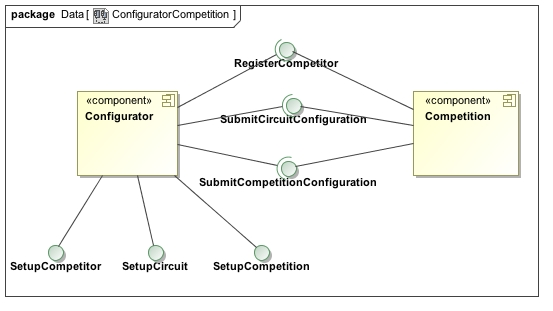
\includegraphics[scale=0.55]{img/InteractionDiagram/Implementation_Diagram__ConfiguratorCompetition.jpg}
\caption{Protocol / Interface diagram - Configurator/Competition}
\end{figure}
\end{center}
Al livello pi\`{u} alto della fase di configurazione c'\`{e} la componente \emph{Configurator}, la quale viene utilizzata per impostare i parametri
relativi alla \emph{Competition}. Tali parametri vengono prima impostati dall'utente %(o letti da file) 
tramite le interfacce \textbf{SetupCompetitor},
\textbf{SetupCompetition} e \textbf{SetupCircuit} e successivamente inviati alla componente \emph{Competition} per l'inizializzazione.\\
\textbf{RegisterCompetitor} \`{e} utilizzata una volta per ogni concorrente da iscrivere.
\clearpage
\subsubsection{Competition-Competitor}
\begin{center}
\begin{figure}[h!]
	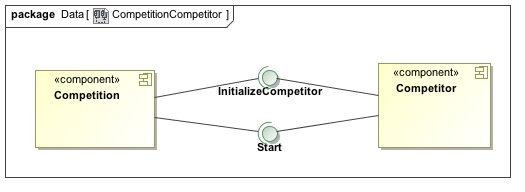
\includegraphics[scale=0.55]{img/InteractionDiagram/Implementation_Diagram__CompetitionCompetitor.jpg}
\caption{Protocol / Interface diagram - Competition/Competitor}
\end{figure}
\end{center}
L'interazione fra la \emph{Competition} e il \emph{Competitor} avviene, come per le altre interazioni \emph{Competition}-componente, in fase di configurazione
e avvio. La \emph{Competition} si occupa di ricevere i parametri relativi a ogni \emph{Competitor} dal \emph{Configurator} (come verr\`{a} spiegato fra poco) per 
poi inizializzare il competitor. Quando tutti i concorrenti sono pronti e anche i \emph{Box}, l'interfaccia \textbf{Start} verr\`{a} utilizzata per dare il
via ai concorrenti.
\subsubsection{Competition-Monitor}
\begin{center}
\begin{figure}[h!]
	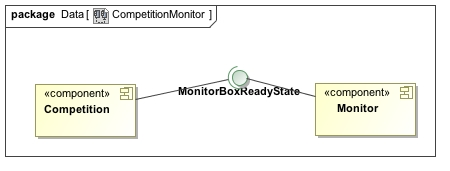
\includegraphics[scale=0.55]{img/InteractionDiagram/Implementation_Diagram__CompetitionMonitor.jpg}
\caption{Protocol / Interface diagram - Competition/Monitor}
\end{figure}
\end{center}
L'interazione \emph{Competition}-\emph{Monitor} riguarda solo una piccola fase dell'inizializzazione, processo che verr\`{a} esplicato in dettaglio in seguito.
A concorrenti registrati, la \emph{Competition} sfrutter\`{a} un interfaccia offerta dal monitor per sapere quando tutti i \emph{Box} sono pronti e avviati.
L'interfaccia \`{e} l'unica illustrata in figura.
\clearpage
\subsubsection{Competition-Circuit}
\begin{center}
\begin{figure}[h!]
	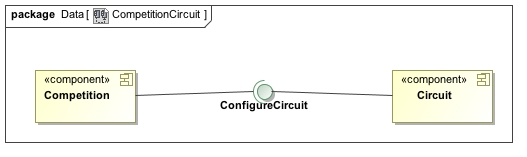
\includegraphics[scale=0.55]{img/InteractionDiagram/Implementation_Diagram__CompetitionCircuit.jpg}
\caption{Protocol / Interface diagram - Competition/Circuit}
\end{figure}
\end{center}
Anche in questo caso, l'interazione \emph{Competition}-\emph{Circuit} si ha in fase di inizializzazione quando le due componenti entrano in contatto
per la configurazione. La \emph{Competition} inizializza cio\`{e} il circuito impostando i parametri che lo caratterizzano, quali:
	\begin{itemize}
		\item numero di checkpoint
		\item caratteristiche dei tratti fra checkpoint (lunghezza, angolo ...)
		\item posizione dei checkpoint di entrata e uscita box
		\item posizione del checkpoint traguardo
	\end{itemize}
\subsubsection{Competition-Stats}
\begin{center}
\begin{figure}[h!]
	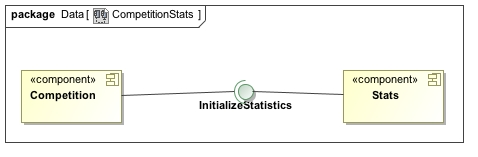
\includegraphics[scale=0.55]{img/InteractionDiagram/Implementation_Diagram__CompetitionStats.jpg}
\caption{Protocol / Interface diagram - Competition/Stats}
\end{figure}
\end{center}
La componente \emph{Stats} ottiene i parametri di configurazione in fase di inizializzazione dalla \emph{Competition}, tramite
\textbf{InitilizeStatistics}.
\clearpage
\subsubsection{Competitor-Stats}
\begin{center}
\begin{figure}[h!]
	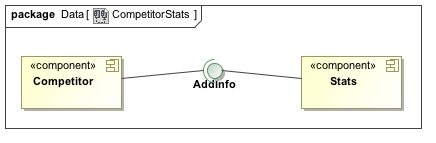
\includegraphics[scale=0.55]{img/InteractionDiagram/Implementation_Diagram__CompetitorStats.jpg}
\caption{Protocol / Interface diagram - Competitor/Stats}
\end{figure}
\end{center}
La componente \emph{Stats} offre al \emph{Competitor} l'interfaccia \textbf{AddInfo} che il concorrente utilizza per fornire costantemente a \emph{Stats}
dati aggiornati riguardo alla gara in corso (dati relativi al singolo concorrente). Ad ogni checkpoint quindi il concorrente manda un aggiornamento
a \emph{Stats} che poi verranno utilizzate per effettuare calcoli di insieme riguardo alla gara o per essere mandate a chi le richiedesse.
\subsubsection{Competitor-Circuit}
\begin{center}
\begin{figure}[h!]
	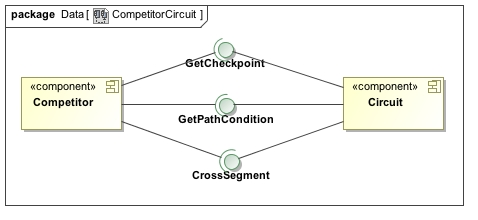
\includegraphics[scale=0.55]{img/InteractionDiagram/Implementation_Diagram__CompetitorCircuit.jpg}
\caption{Protocol / Interface diagram - Competitor/Circuit}
\end{figure}
\end{center}
L'interazione \emph{Competitor}-\emph{Circuit} avviene durante lo svolgimento della competizione. Il concorrente sfrutta le interfacce del \emph{Circuit}
per ottenere informazioni sul circuito e ``informarlo'' degli spostamenti nel corso della gara.\\
\textbf{GetCheckpoint} garantisce che il concorrente ottenga sempre il checkpoint corretto a seconda della posizione corrente.
\textbf{GetPathCondition} permette di ottenere informazioni sulle caratteristiche statiche e dinamiche della tratto da attraversare. Le caratteristiche 
dinamiche sono legate ai concorrenti attualmente presenti sul tratto.
\textbf{CrossSegment} assicura che il tratto possa essere attraversato senza collisioni e che il \emph{Circuit} possa tracciare l'avvenuto passaggio 
dell'auto.
\subsubsection{Monitor-Stats}
\begin{center}
\begin{figure}[h!]
	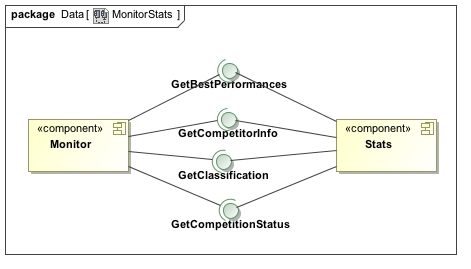
\includegraphics[scale=0.55]{img/InteractionDiagram/Implementation_Diagram__MonitorStats.jpg}
\caption{Protocol / Interface diagram - Monitor/Stats}
\end{figure}
\end{center}
La componente \emph{Monitor} si appoggia a \emph{Stats} per poter reperire le informazioni da essere esposte. Per questo motivo
\emph{Stats} offre un insieme di interfacce finalizzate a fornire i dati grezzi di competizione sotto forma di viste utili alla ``pubblicazione''.\\
\textbf{GetBestPerformance} fornisce i migliori tempi relativi a settori e giro.\\
\textbf{GetCompetitorInfo} reperisce informazioni legate al singolo concorrente, come ad esempio lo stato della macchina ad un determinato istante.\\
\textbf{GetClassification}, come dice il nome, ritorna informazioni legate alla classifica.\\
\textbf{GetCompetitionStatus} espone informazioni legate alla competizione nel suo insieme, come ad esempio la posizione dei concorrenti nel circuito
in un determinato istante di tempo.
\clearpage
\subsubsection{Configurator-Box}
\begin{center}
\begin{figure}[h!]
	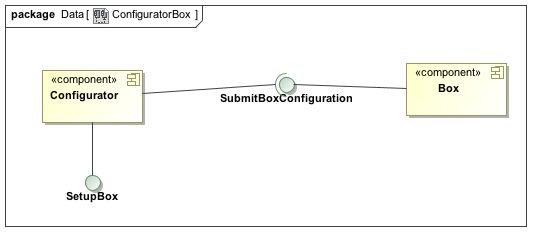
\includegraphics[scale=0.55]{img/InteractionDiagram/Implementation_Diagram__ConfiguratorBox.jpg}
\caption{Protocol / Interface diagram - Configurator/Box}
\end{figure}
\end{center}
La componente \emph{Configurator} offre anche la possibilit\`{a} di configurare un \emph{Box}. Per questo motivo il \emph{Box} espone un'interfaccia
da utilizzare per sottomettere i parametri di configurazione. 
\subsubsection{Box-Monitor}
\begin{center}
\begin{figure}[h!]
	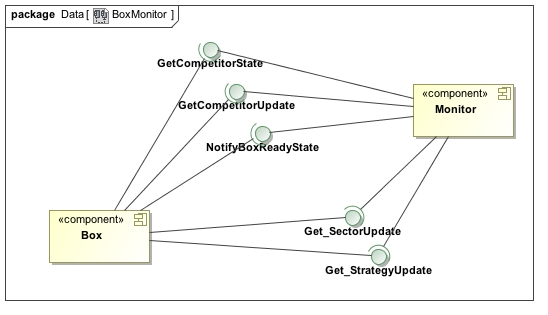
\includegraphics[scale=0.55]{img/InteractionDiagram/Implementation_Diagram__BoxMonitor.jpg}
\caption{Protocol / Interface diagram - Box/Monitor}
\end{figure}
\end{center}
La prima interazione che la componente \emph{Box} ha con il \emph{Monitor} \`{e} in fase di inizializzazione della gara. 
La sequenza di azioni verr\`{a} esplicata
dettagliatamente in seguito, per ora basti sapere che il \emph{Box}, una volta configurato e pronto per monitorare 
la gara ed elaborare i dati del suo
concorrente, dovr\`{a} mandare una notifica tramite la componente \emph{Monitor} utilizzando \textbf{NotifyBoxReadyState}.\\
Le rimanenti due interfacce offerte dal \emph{Monitor} al \emph{Box} sono utilizzate per reperire informazioni sullo stato del 
concorrente (livello di benzina rimasta, usura gomme...) e
aggiornamenti riguardo al posizionamento e tempi del concorrente durante la gara.\\
Vi sono poi altre due interfacce offerte dal \emph{Box} al \emph{Monitor}. Per quanto possa sembrare un po' paradossale, l'architettura
acquisisce senso se si pensa che la componente \emph{Monitor}, ad alto livello, \`{e} stata pensata per pubblicare informazioni. Tali
informazioni possono riguardare il singolo concorrente e quindi essere utili al \emph{Box}. Altre possono invece riguardare il \emph{Box} e 
i suoi calcoli per essere esposte ad un utente (per esempio). Le due interfacce offerte dal \emph{Box} infatti servono per ottenere
aggiornamenti sulle operazioni interne del \emph{Box} qualora esse dovessero essere esposte ad un qualunque client. Come vedremo pi\`{u}
in dettaglio in seguito, questa componente \`{e} in realt\`{a} costituita da due sotto-componenti, una dedicata a \emph{Competition} e l'altra a
\emph{Box}.
\subsubsection{Screen-Monitor}
\begin{center}
\begin{figure}[h!]
	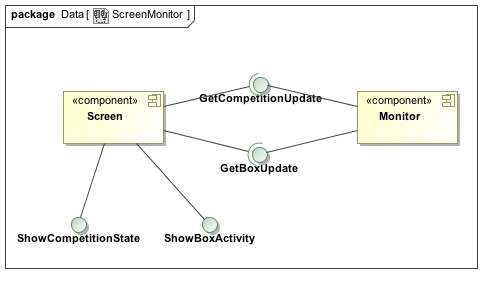
\includegraphics[scale=0.55]{img/InteractionDiagram/Implementation_Diagram__ScreenMonitor.jpg}
\caption{Protocol / Interface diagram - Screen/Monitor}
\end{figure}
\end{center}
La componente \emph{Screen} comunica con il \emph{Monitor} per ottenere informazioni utili da esporre graficamente all'utente. Tali
informazioni possono riguardare la competizione in senso globale, oppure essere legate ai singoli concorrenti.
\subsubsection{Competitor-Box}
\begin{center}
\begin{figure}[h!]
	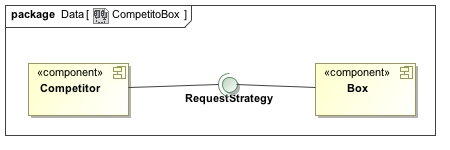
\includegraphics[scale=0.55]{img/InteractionDiagram/Implementation_Diagram__CompetitoBox.jpg}
\caption{Protocol / Interface diagram - Competitor/Box}
\end{figure}
\end{center}
Man mano che la competizione procede, il \emph{Box} colleziona i dati di gara del rispettivo concorrente per calcolarne medie e statistiche. 
A partire da queste informazioni produce una nuova strategia ogni giro. Per questo offre un'interfaccia \textbf{RequestStrategy} che il concorrente
utilizza nel corso della gara per ottenere suggerimenti utili per proseguire. La strategia fornita dal \emph{Box} potrebbe anche richiedere 
un pitstop per un rifornimento benzina e cambio gomme.
% Strategia adottata per la correttezza temporale
\subsection{Strategia di simulazione}
\label{strategia_simulazione}
In questa sezione viene spiegata la strategia che \`{e} stata adottata per ottenere una simulazione realistica della gara. Le problematiche da 
affrontare sono gi\`{a} state discusse nel capitolo \ref{problematiche_concorrenza}.\\ 
La soluzione prevede l'esistenza di concorrenti che simultaneamente percorrono il circuito e un insieme di entit\`{a} di supporto per evitare 
i problemi visti. Tali entit\`{a} sono:
\begin{itemize}
  \item \textbf{coda al checkpoint}: ogni checkpoint introduce tratti di circuito con caratteristiche diverse rispetto a quello precedente.
	      \`{E} quindi possibile che da un tratto a molteplicit\`{a} 5 si passi ad uno a molteplicit\`{a} 3. L'accesso a tale tratto va quindi
	      regolato per evitare situazioni anomale. La coda \`{e} ordinata in base ai tempi segnati (ulteriori dettagli in seguito).
  \item \textbf{istante di arrivo}: \`{e} l'istante in cui il concorrente \`{e} previsto arrivare. Indica l'istante reale di arrivo e dipende
	      dal tempo di attraversamento (oltre che dal tempo accumulato fino a quel momento).
  \item \textbf{istante limite di arrivo previsto}: \`{e} l'istante in cui il concorrente arriverebbe sotto ipotesi ottimistiche al massimo. 
	      E' impossibile che il concorrente possa arrivare ad un checkpoint prima di questo istante. 
  \item \textbf{flag ``arrivato''}: ogni posizione della coda di un checkpoint \`{e} caratterizzata anche da questa flag. Se \`{e} settata, significa
	      che il concorrente in tale posizione \`{e} effettivamente in attesa sul checkpoint pronto ad attraversare. Altrimenti significa
	      che \`{e} fisicamente su un altro tratto e che il tempo segnato \`{e} un tempo limite (e non l'istante di arrivo effettivo).
  \item \textbf{istante di liberazione traiettoria}: ogni traiettoria presente in un tratto \`{e} contrassegnata da questo tempo. Se un concorrente
	      arriva all'istante 42.0, la traiettoria in quel momento \`{e} libera e calcola un tempo di attraversamento di 3.0, l'istante di liberazione
	      della traiettoria sar\`{a} 42.0+3.0 = 45.0. 
\end{itemize}
Detto questo \`{e} possibile vedere l'algoritmo per l'attraversamento di un tratto dal momento in cui il concorrente arriva fisicamente ad un checkpoint
fino al raggiungimento di quello successivo.\\
\emph{Premessa}: un concorrente controlla la sua posizione su una coda ogni volta che essa viene riordinata.\\
\emph{Precondizione}: il concorrente ha gi\`{a} segnato il suo tempo di arrivo effettivo sulla coda del checkpoint che vuole attraversare.
\begin{enumerate}
\item il concorrente setta la flag ``arrivato'' nella coda del checkpoint sulla posizione a lui riservata;
\item controlla in che posizione \`{e} nella coda;
\item se non \`{e} primo, attende di essere primo;
\item quando \`{e} primo, richiede l'insieme di traiettorie da cui \`{e} costituito il tratto;
\item valutando gli istanti di liberazione e le caratteristiche della traiettorie, decide quale sia quella che garantisce l'arrivo al checkpoint
successivo all'istante di tempo pi\`{u} vicino.
\item aggiunge il tempo di attraversamento calcolato (in base alle caratteristiche dell'auto e alla strategia) al tempo di liberazione del tratto o, 
se il tempo di liberazione segnato \`{e} minore dell'istante di arrivo del concorrente, segna come istante di liberazione \emph{istante di arrivo}+\emph{tempo
di attraversamento} (poich\`{e} significa che la traiettoria era gi\`{a} stata liberata all'arrivo del concorrente). Altrimenti segnerà \emph{tempo segnato+tempo di attraversamento}.
\item segna il tempo di arrivo effettivo (dipendente chiaramente dal tempo segnato sulla traiettoria) sulla coda del checkpoint successivo, che verr\`{a} \textbf{riordinata} in base al nuovo tempo.
\item segna il tempo di arrivo limite su tutte le altre code, da quella successiva al checkpoint che si sta per raggiungere a quella del checkpoint
appena attraversato. Ad ogni aggiornamento del tempo limite, la coda viene \textbf{riordinata}.
\item delay per fini di simulazione;
\item ritorna al passo uno per il checkpoint successivo;
\end{enumerate}
La strategia adottata si presta a simulare la corsa tenendo in considerazione ad ogni istante le auto presenti sulla pista e sui tratti senza comportamenti
anomali. Questo perch\`{e}:
\begin{itemize}
\item \emph{quando un concorrente \`{e} primo sulla coda ed effettivamente presente sulla coda, nessun concorrente potr\`{a} diventare primo finch\`{e} non sia il concorrente
stesso attualmente primo a riordinare la lista}. Questo perch\`{e}, i tempi limite segnati sono i tempi minimi. Se il tempo effettivo del concorrente attualmente
primo \`{e} inferiore a tutti tempi limite, essendo minimi, non potranno diventare pi\`{u} piccoli successivamente. Se nel frattempo qualcun altro arriva sul 
checkpoint, esso segner\`{a} un tempo effettivo. Essendo il tempo effettivo per definizione maggiore o uguale al tempo limite, non sar\`{a} possibile che un tempo
effettivo segnato successivamente possa essere minore di quello del concorrente attualmente primo.
\item \emph{quando un concorrente valuta le traiettorie, lo sta facendo in modo esclusivo}. Questa condizione \`{e} assicurata dal punto precedente. Mentre il 
concorrente valuta le traiettorie, nessuno pu\`{o} diventare primo e effettuare una valutazione parallela delle stesse traiettorie. Il concorrente riordiner\`{a}
la lista solo a traiettoria valutata, scelta e segnata con istante di liberazione, permettendo ad un altro concorrente di procedere.
\item \emph{non possono esserci teletrasporti}. Prendendo il caso peggiore, ovvero un tratto ad una traiettoria, un segnale di teletrasporto avvenuto sarebbe
che nel checkpoint N il concorrente A abbia tempo di arrivo effettivo 4.0 e il concorrente B 7.0. Dopo l'attraversamento di entrambi dovrebbe esserci nella 
coda del checkpoint N+1 il concorrente B con 6.0 in prima posizione (ad esempio) e A con 8.0 a seguire. Il che significherebbe che in qualche modo B, nonostante
abbia avuto accesso al tratto dopo A, sia riuscito lo stesso a sorpassarlo arrivando primo al checkpoint dopo. La cosa non pu\`{o} succedere. Per i punti spiegati
prima, quando A arriva primo effettivo sulla coda del checkpoint N, potr\`{a} eseguire la valutazione delle traiettorie in modo esclusivo. Verr\`{a} quindi segnato
un istante di liberazione sull'unica traiettoria disponibile maggiore o uguale a 4.0. Supponiamo 8.0. Verr\`{a} quindi segnato 8.0 nella coda del checkpoint N+1. A
seguire verranno segnati $8.0+\epsilon$ su tutti gli altri tratti, fino al tratto N di nuovo dove la coda verr\`{a} riordinata e B risulter\`{a} primo effettivo.
Ora, supponiamo (caso pessimo) che A non possa eseguire per un bel po' di tempo. B diventa primo su N, valuta la traiettoria e segna l'istante di liberazione.
Tale istante non potr\`{a} essere minore di 8.0, poich\`{e} \`{e} stato il tempo segnato da A. Quindi, qualunque tempo di arrivo effettivo segnato al checkpoint
N+1, sar\`{a} maggior di 8.0. Quindi B finir\`{a} in una posizione nella coda meno prioritaria rispetto ad A. In qualunque momento A venga riattivato quindi, sar\`{a}
sicuro di non trovarsi B inaspettatamente davanti.
\item \emph{un numero maggiore di o uguale a 2 di concorrenti eseguono in modo concorrente}: prendendo il caso precedente, dove A ha appena finito di valutare le
traiettorie del tratto N. A segna un tempo pari a 8.0 effettivo sulla coda N+1 e $N+1+\epsilon$ (crescente) su tutti gli altri fino ad N di nuovo. Supponiamo
B abbia segnato un tempo inferiore a $N+1+max(\epsilon)$ su N. B valuter\`{a} le traiettorie del tratto N. Nel frattempo A \`{e} primo sul tratto N+1 (assumendo
che B avesse segnato un tempo limite comunque pi\`{u} basso del tempo effettivo di A). A valuter\`{a} le traiettorie
''simultaneamente'' a B. Abbiamo quindi un sistema con task concorrenti.
\end{itemize}
Del rientro ai box non se ne \`{e} ancora discusso per evitare di rendere pi\`{u} confusionaria la spiegazione. Comunque la cosa non costituisce
un grande problema: vi saranno due checkpoint speciali, quello esattamente prima della corsia dei box e quello subito all'uscita dei box.
Quando un concorrente arriva sul checkpoint precedente ai box, richiede delle informazioni di strategia ai box. Se tali informazioni
richiedono un rientro, il concorrente prender\`{a} il tratto dei box. Il box \`{e} poi rappresentato da un checkpoint come tutti gli altri nel circuito.
Tale checkpoint introduce il tratto di uscita dai box, che porter\`{a} al checkpoint di uscita (nel circuito).\\
I tratti nella corsia dei box hanno molteplicit\`{a} pari al numero di concorrenti. Questo perch\`{e} i concorrenti vanno alla stessa
velocit\`{a} nelle corsie dei box e potenzialmente tutti insieme (uno dietro l'altro), quindi non possono avvenire sorpassi. L'unica ipotesi di
sorpasso \`{e} data dalla velocit\`{a} che un concorrente richiede per il rifornimento e il cambio gomme. Tale tempo influir\`{a} sull'istante di arrivo
che verr\`{a} segnato nel checkpoint di uscita.
% Dimostrazione dell'assenza di stallo
\subsection{Assenza di stallo}
Le situazioni di stallo non si verificano per i seguenti motivi. Ragionando per assurdo, uno stallo si potrebbe verificare se:
una macchina A attende la prima posizione nella coda associata al tratto 3 (per esempio). 
Nel frattempo Un concorrente B \`{e} in attesa sulla coda associata al tratto 2. Ma B risulta prima di A nella coda 3 e A 
risulta prima di B nella coda 2 e il tratto 2-3 possiede una sola traiettoria.\\
lo stallo porterebbe ad una contraddizione.\\
\begin{proof}
\textcolor{white}{42}\\
\emph{Premessa: tempo(NX) $\rightarrow$ tempo del concorrente X segnato sul checkpoint N.}\\
	Se nella coda 2 ci sono A in testa seguita da B, avremo che $tempo(2A)<tempo(2B)$, poich\`{e} l'ordine della coda \`{e} 
	determinato dai tempi di arrivo segnati.
	Se A \`{e} in attesa sulla coda 3, vuol dire che avr\`{a} aggiornato per ultima la coda 3-1, ovvero 2, e di conseguenza $tempo(2A)>tempo(3A)$.
	B invece \`{e} in attesa effettiva sulla coda 2, quindi avr\`{a} aggiornato la coda del tratto successivo con un valore dato da $t(2B)+ \delta t$, 
	con $ \delta t$ un valore minimo diverso da zero previsto per l'attraversamento da 2 a 3. Quindi $tempo(2B)<tempo(3B)$.
	L'ipotesi di stallo prevede che nella coda 3 vi sia prima B e poi A, quindi $tempo(3B)<tempo(3A)$.
	Avremo quindi:\\

	$tempo(3A)<tempo(2A)<tempo(2B)<tempo(3B)<tempo(3A)$\\\\
	che \`{e} una contraddizione, quindi la situazione non si pu\`{o} verificare.
\end{proof}
\newpage
%%% Architettura in dettaglio %%
\section{Architettura in dettaglio}
Si spiegher\`{a} ora con maggior dettaglio l'architettura di sistema, esplicando come le principali classi implementate svolgano le funzionalit\`{a}
esposte dalle interfacce illustrate nel capitolo precedente.
\subsection{Diagrammi delle classi}
\subsubsection{Competition}
\begin{center}
\begin{figure}[h!]
	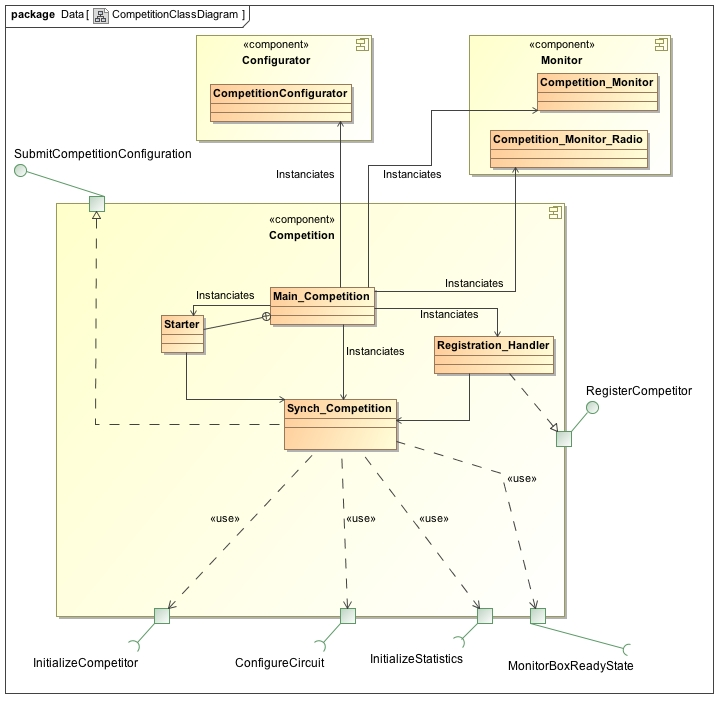
\includegraphics[scale=0.50]{img/ClassDiagrams/CompetitionClassDiagram.jpg}
\caption{Class diagram - Competition}
\end{figure}
\end{center}
La \emph{Competition} \`{e}, come gi\`{a} accennato, una componente di init.\\
Il tutto ha inizio a partire da \textbf{Main\_Competition} che, come dice il nome, \`{e} l'unit\`{a} di avvio.\\
\textbf{Main\_Competition} si occupa di istanziare gli oggetti necessari all'avvio e configurazione della competizione. Per la configurazione
vengono istanziati \textbf{RegistrationHandler} e \textbf{CompetitionConfigurator} (della componente \emph{Configurator}).
Per l'avvio invece \textbf{Starter}. \\
Ad orchestrare la scena, un unica istanza del \textbf{Synch\_Competition} condivisa fra le altre 3 unit\`{a}. Il loro scopo \`{e}:
\begin{itemize}
\item \textbf{Synch\_Competition}, \`{e} una risorsa protetta che gestisce l'accesso in mutua esclusione alla configurazione della competizione
e dell'inizializzazione dei concorrenti. La risorsa assicura tramite \emph{entry} a guardia booleana
che avvengano in ordine prima la configurazione
della competizione (da parte del \textbf{CompetitionConfigurator}) e poi la registrazione dei concorrenti (per opera del \textbf{RegistrationHandler}).
Questo vincolo \`{e} dato dal fatto che alcune impostazioni di competizioni devono essere fornite ai box dopo la configurazione del concorrente, 
come ad esempio il numero di lap. Inoltre fra i parametri configurabili vi \`{e} anche il numero massimo di partecipanti alla gara. Di conseguenza
\`{e} prima necessario conoscere il limite per poi poter regolare il flusso di registrazioni.\\
Durante la fase di configurazione (metodo \underline{Configure}), vengono inizializzati \emph{Circuit} e \emph{Stats} tramite le interfacce
illustrate nel diagramma.\\
A configurazione di competizione avvenuta, verr\`{a} aperta le entry\\ \underline{Register\_NewCompetitor}, utilizzata dal \textbf{RegistrationHandler}
per registrare i vari concorrenti. Ad ogni invocazione verr\`{a} inizializzato un concorrente (\textbf{TaskCompetitor}) con un iteratore al circuito
e le impostazioni passate in input. Il task del concorrente cos\`{i} istanziato rimarr\`{a} in attesa dello ``start''.\\
Oltre alla funzionalit\`{a} di configurazione, questa classe offre anche la funzionalit\`{a} di avvio (metodo \underline{Start}).
Tale entry si aprir\`{a} solo quando tutti i concorrenti previsti sono stati iscritti. Viene invocata dall'unit\`{a} \textbf{Starter}.
Il metodo mette il task richiedente in attesa sulla risorsa \textbf{StartHandler} (componente \emph{Monitor}) sull'entry \underline{MonitorBoxReadyState}.
Quanto tutti i box avranno dato il loro ok (maggiori dettagli a seguire), il thread potr\`{a} continuare la sua esecuzione e passare allo \underline{Start}
di tutti i concorrenti in attesa di partire.
\item \textbf{Starter} \`{e} il task finalizzato a gestire l'avvio della competizione. Una volta avviato dal main, il task utilizza il metodo \underline{Ready}
offerto dal package \emph{Competition} per manovrare l'avvio. All'interno del metodo, prima si mette in attesa che tutti i concorrenti
si siano iscritti (utilizzando il metodo \underline{Wait} del singleton di \textbf{Synch\_Competition}) per poi invocare il metodo \underline{Start} dello
stesso \textbf{Synch\_Competition}, descritto poche righe pi\`{u} sopra.
\item \textbf{RegistrationHandler} \`{e} l'oggetto che rimane in attesa di concorrenti. Pi\`{u} precisamente, \`{e} un server dedicato ad accogliere
le richieste di registrazione dei concorrenti. Con il supporto di Polyorb \`{e} possibile invocare questo oggetto da remoto. Ad ogni richiesta,
vengono salvati i parametri di configurazione in un file xml il cui nome e locazione verranno passati a \textbf{Synch\_Competition} per
 effettuare il resto delle procedure di inizializzazione del concorrente. Di ritorno ci saranno l'ID del concorrente, il numero di lap,
la lunghezza del circuito e il corbaloc 
del \textbf{Competition\_Monitor} che il \emph{Box} dovr\`{a} utilizzare per rimanere sincronizzato sugli sviluppi del rispettivo concorrente.
\end{itemize}
\subsubsection{Competitor}
\begin{center}
\begin{figure}[h!]
	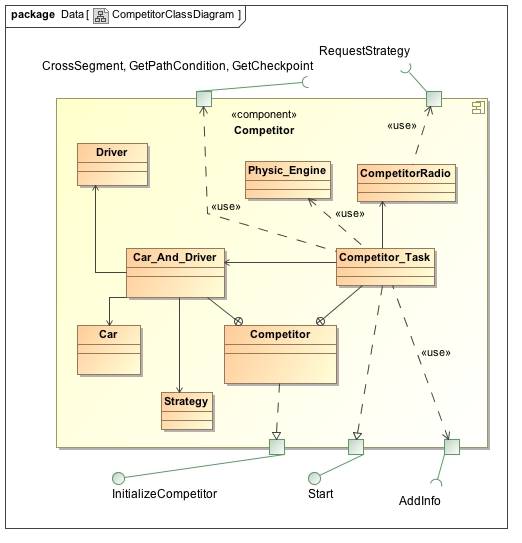
\includegraphics[scale=0.50]{img/ClassDiagrams/CompetitorClassDiagram.jpg}
\caption{Class diagram - Competitor}
\end{figure}
\end{center}
L'unit\`{a} principale del \emph{Competitor} \`{e} il \textbf{TaskCompetitor}. \`{E} la risorsa attiva che si occupa di percorrere la pista e valutare
la traiettoria ottima in base alle condizioni del tratto e dei competitor presenti nelle vicinanze. Le informazioni statiche del concorrente
sono contenute in \textbf{Driver}. \textbf{Car} mantiene alcune caratteristiche statiche sulla macchina e altre dinamiche, come il livello
di benzina e l'usura delle gomme. \textbf{Strategy} mantiene le seguenti informazioni:
\begin{itemize}
%\item Tipo gomme
\item Stile di guida
\item Numero di giri al pitstop (se 0, bisogna rientrare al pitstop)
\item Durata del pitstop (nel caso il pitstop sia avvenuto)
\item Livello di Gas (dopo il pitstop in caso sia avvenuto)
\end{itemize}
\textsc{Stile di guida} e \textsc{Numero di giri al pitstop} vengono aggiornate ad ogni giro, \textsc{Durata del pitstop}
e \textsc{Livello di gas} vengono tenute in considerazione solo in caso di pitstop. Il livello di gas viene usato per aggiornare
le impostazioni di \textbf{Car} (le gomme vengono automaticamente messe a nuovo). 
La durata del pitstop viene usata per aggiornare correttamente il tempo di arrivo segnato nel checkpoint di uscita
dai box.\\
Quando un concorrente si trova sul checkpoint prima della corsia dei box, effettua una chiamata al \emph{Box} tramite la \textbf{CompetitorRadio}
per richiedere una strategia aggiornata. Se la strategia tornata contiene un numero di giri al pitstop pari a 0, il \textbf{TaskCompetitor}
valuter\`{a} e percorrer\`{a} la corsia dei box invece che quella del circuito, per poter effettuare il pitstop.\\\\
Il \textbf{TaskCompetitor} e tutte le unit\`{a} associate vengono inizializzate in fase di init tramite i seguenti metodi offerti dal package
\textbf{Competitor}:
\begin{itemize}
\item \underline{Configure\_Driver}
\item \underline{Configure\_Car}
\item \underline{Costruttore \textbf{TaskCompetitor}}
\end{itemize}
\newpage
\subsubsection{Circuit}
\begin{center}
\begin{figure}[h!]
	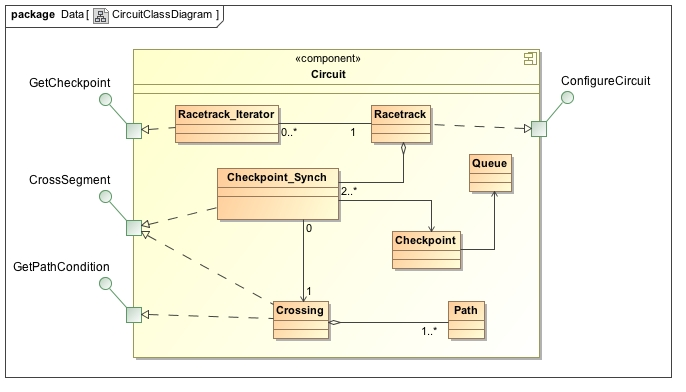
\includegraphics[scale=0.50]{img/ClassDiagrams/CircuitClassDiagram.jpg}
\caption{Class diagram - Circuit}
\end{figure}
\end{center}
Il circuito prende forma a partire da \textbf{Racetrack}. Questa unit\`{a} si occupa di leggere e parsare il file xml dato in input e ricavarne
i parametri per la creazione del circuito. Il file XML descrittore del circuito elenca i checkpoint presenti in ogni settore (che sono
3 costanti) e per ognuno specifica le caratteristiche del tratto di pista a seguire:
\begin{itemize}
  \item lunghezza
  \item angolo
  \item molteplicit\`{a} (numero di concorrenti che possono attraversare contemporaneamente il tratto)
  \item grip, ovvero aderenza sul tratto
\end{itemize}
Vi sono inoltre 3 checkpoint che dovranno avere uno dei seguenti attributi booleani:
\begin{itemize}
\item goal, ovvero il checkpoint \`{e} il primo della pista
\item prebox, ovvero dal checkpoint \`{e} possibile raggiungere i box
\item exitbox, ovvero il checkpoint di arrivo una volta fuori dalla corsia dei box
\end{itemize}
Dati questi parametri, vengono inizializzati tutti i checkpoint stabiliti ed inseriti in un array chiamato \textbf{Racetrack}. Questo
sar\`{a} l'array iterato dal \textbf{Race\_Iterator}.\\

Ogni checkpoint \`{e} del tipo \textbf{Checkpoint}, il quale contiene tutte le informazioni elencate in precedenza oltre ad una coda per gestire
i concorrenti che tentano di accedere al tratto. Il \textbf{Checkpoint} \`{e} poi inserito in una struttura protetta denominata 
\textbf{Checkpoint\_Synch} finalizzata a regolare l'accesso in mutua esclusione. La risorsa inoltre incapsula la lista di \textbf{Path}
che costituiscono il tratto associato al checkpoint. Infine offre una serie di metodi da utilizzarsi per interagire con le risorse sottostanti.\\
I \textbf{Path} appena accennati vengono generati in fase di creazione del \textbf{Checkpoint} a partire dalle informazioni di base
reperite dal file di configurazione. Vengono generati tanti \textbf{Path} quanto la molteplicit\`{a} impostata del tratto. Ogni \textbf{Path} 
riceve valori di lunghezza che possono variare. Bisogna assicurare 1.5 m di larghezza per ogni macchina (approssimativamente). La prima
riceve i valori di base e viene virtualmente posizionata su un bordo del tratto. Le altre vengono posizionate man mano una di fianco all'altra,
quindi la lunghezza della traiettoria cresce in rapporto alla distanza dalla prima e all'angolo del tratto. Tutti i \textbf{Path} di un tratto
vengono incapsulati in una risorsa protetta denominata \textbf{Crossing} che ne regola l'accesso in mutua esclusione e offre i metodi di 
accesso pubblici.\\
Infine viene creata una corsia dei box coerente con la distanza fra i checkpoint ``prebox'' e l'``exitbox''. I tratti prima e dopo il checkpoint
dei box sono a molteplicit\`{a} uguale al numero di concorrenti. Questo perch\`{e} potenzialmente ai box potrebbero esserci contemporaneamente tutte
le auto. Inoltre si \`{e} deciso di posizionare il checkpoint del box in coincidenza con il traguardo. Quindi ogni box \`{e} anche un goal.\\\\
Verranno ora elencati metodi pi\`{u} rilevanti esposti dal \textbf{Checkpoint\_Synch} 
per poter mettere in pratica la strategia di attraversamento descritta nella sezione \ref{strategia_simulazione}:
\begin{description}
\item{\textbf{procedure Signal\_Arrival(CompetitorID\_In : INTEGER)}}\\
Il metodo marca nella coda del checkpoint l'arrivo effettivo del concorrente;
\item{\textbf{procedure Signal\_Leaving(CompetitorID\_In : INTEGER)}}\\
Il metodo marca nella coda del checkpoint l'uscita del concorrente;
\item{\textbf{procedure Set\_ArrivalTime(CompetitorID\_In : INTEGER; Time\_In : FLOAT)}}\\
Il metodo segna il tempo previsto di arrivo del concorrente nella coda del checkpoint;
\item{\textbf{procedure Remove\_Competitor(CompetitorID\_In : INTEGER)}}\\
Il metodo rimuove il competitor dalla coda. Ci\`{o} significa che l'id e il tempo del competitor non apparir\`{a} pi\`{u}
nella coda. Questo metodo \`{e} utilizzato, per esempio, quando un concorrente finisce la gara prima di altri
e deve quindi liberare i checkpoint per evitare di creare starvation;
\item{\textbf{function Get\_Time(CompetitorID\_In : INTEGER) return FLOAT}}
La funzione ritorna il tempo segnato sulla coda del concorrente con ID dato in input;
\item{\textbf{entry Wait\_Ready(Competitor\_ID : INTEGER)}}
Nel momento in cui un concorrente arriva fisicamente su un checkpoint, dopo aver marcato il suo arrivo
utilizza questo metodo per sapere quando arriva il suo turno per attraversare (viene cio\`{e} posizionato nella prima posizione della coda);
\item{\textbf{procedure Get\_Paths(Paths2Cross : out CROSSING\_POINT;  Go2Box : BOOLEAN)}}
Quando il concorrente sa di essere primo sulla coda del \textbf{Checkpoint}
(in seguito all'invocazione del metodo \underline{Wait\_Ready}), potr\`{a} invocare questa procedura per
ottenere l'insieme di \textbf{Path} che costituiscono il tratto e procedere alla valutazione. Il booleano ``Go2Box'', se valorizzato a ``true'',
impone al \textbf{Checkpoint\_Synch} di tornare (se presente) l'insieme di \textbf{Path} relativi alla corsia dei box.
Si \`{e} sicuri che nessuno star\`{a} effettuando operazioni sul tratto nel frattempo perch\`{e} tale azione da parte
degli altri concorrenti non \`{e} ammissibile fino a che il \textbf{Competitor} corrente non abbia segnalato la sua partenza dal checkpoint
tramite \underline{Signal\_Leaving}.
\end{description}
I metodi della risorsa \textbf{Crossing} invece servono a ritornare le caratteristiche di ogni \textbf{Path} (a partire dall'indice) e a aggiornare
l'istante temporale segnato nel path.\\\\
Infine sono offerti un insieme di metodi da utilizzare insieme al \textbf{RaceTrack\_Iterator} per navigare iterare il circuito. I metodi sono pi\`{u}
rilevanti sono:
\begin{description}
\item{\textbf{procedure Get\_CurrentCheckpoint\\(RaceIterator : in out RACETRACK\_ITERATOR;\\ CurrentCheckpoint : out CHECKPOINT\_SYNCH\_POINT)}}\\
Per ottenere il checkpoint correntemente ``puntato'' dall'iteratore;
\item{\textbf{procedure Get\_NextCheckpoint\\(RaceIterator : in out RACETRACK\_ITERATOR;\\ NextCheckpoint : out CHECKPOINT\_SYNCH\_POINT)}}\\
Per ottenere il checkpoint successivo. Nota Bene: il checkpoint dei box non \`{e} previsto essere ritornato da questo metodo. Per ottenere il
checkpoint dei box \`{e} necessario utilizzare \underline{Get\_BoxCheckpoint};
\item{\textbf{procedure Get\_PreviousCheckpoint\\(RaceIterator : in out RACETRACK\_ITERATOR;\\ PreviousCheckpoint : out CHECKPOINT\_SYNCH\_POINT)}}\\
Per ottenere il checkpoint precedente, con le stesse regole del metodo precedente;
\item{\textbf{procedure Get\_ExitBoxCheckpoint\\(RaceIterator : in out RACETRACK\_ITERATOR;\\ ExitBoxCheckpoint : out CHECKPOINT\_SYNCH\_POINT)}}\\
Per ottenere il checkpoint all'uscita della corsia dei box;
\item{\textbf{procedure Get\_BoxCheckpoint\\(RaceIterator : in out RACETRACK\_ITERATOR;\\ BoxCheckpoint : out CHECKPOINT\_SYNCH\_POINT)}}\\
Per ottenere il checkpoint del box;
\item{\textbf{function Get\_Position\\(RaceIterator : RACETRACK\_ITERATOR) return INTEGER}}\\
Per tornare la posizione corrente dell'iteratore.
\end{description}
Non \`{e} stato necessario inserire \textbf{Racetrack} o il suo iteratore in una risorsa protetta perch\`{e} ogni concorrente dispone della
sua copia dell'\textbf{Racetrack\_Iterator}.
\newpage
\subsubsection{Stats}
\begin{center}
\begin{figure}[h!]
	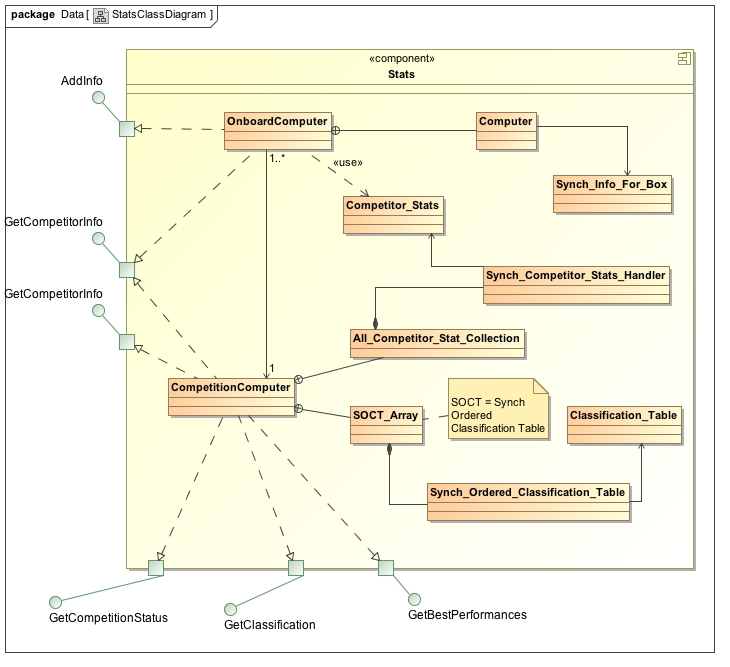
\includegraphics[scale=0.50]{img/ClassDiagrams/StatsClassDiagram.jpg}
\caption{Class diagram - Stats}
\end{figure}
\end{center}
La componente \emph{Stats} \`{e} implicitamente suddivisa in 2 sotto-componenti: \textbf{OnboardComputer} e \textbf{CompetitionComputer}. 
Prima di discutere dei dettagli delle due, \`{e} necessario introdurre la struttura di una risorsa che viene utilizzata come
pacchetto per il trasporto degli aggiornamenti tra \emph{Competitor}, \textbf{OnboardComputer} e \textbf{CompetitionComputer}. La risorsa \`{e} 
un tipo record denominato \textbf{Competitor\_Stats}, contenente i seguenti dati:
\begin{itemize}
      \item\textbf{Time : FLOAT;}\\l'istante a cui fa riferimento l'aggiornamento
      \item\textbf{Checkpoint : INTEGER;}\\il checkpoint che introduceva il tratto che \`{e} stato attraversato (completato) all'istante \textsc{Time}
      \item\textbf{LastCheckInSect : BOOLEAN;}\\se true, il checkpoint \`{e} l'ultimo di un settore
      \item\textbf{FirstCheckInSect : BOOLEAN;}\\su true, il checkpoint \`{e} il primo del settore
      \item\textbf{Sector : INTEGER;}\\il settore a cui appartiene il checkpoint
      \item\textbf{Lap : INTEGER;}\\la lap in cui a cui l'aggiornamento fa riferimento
      \item\textbf{GasLevel : FLOAT;}\\il livello di gas presente nel serbatoio al momento in cui il tratto \`{e} stato attraversato (completato)
      \item\textbf{TyreUsury : PERCENTAGE;}\\la percentuale di usura gomme al momento in cui il tratto \`{e} stato attraversato (completato)
      \item\textbf{BestLapNum : INTEGER;}\\la miglior lap fatta dal concorrente dall'inizio della gara all'istante \textsc{Time}
      \item\textbf{BestLaptime : FLOAT;}\\il tempo della miglior lap fatta dal concorrente dall'inizio della gara all'istante \textsc{Time}
      \item\textbf{BestSectorTimes : FLOAT\_ARRAY(1..3);}\\ogni indice dell'array indica un settore (quindi indice 1 indica il settore 1). Detto ci\`{o},
      l'array contiene il miglior tempo fatto dal concorrente per ogni settore dall'inizio della gara all'istante \textsc{Time}
      \item\textbf{MaxSpeed : FLOAT;}\\la massima velocit\`{a} raggiunta dall'inizio della gara all'istante \textsc{Time}
      \item\textbf{PathLength : FLOAT;}\\la lunghezza della traiettoria scelta per attraversare il tratto
\end{itemize}
Ora vediamo pi\`{u} dettagliatamente le due sotto-componenti accennate precedentemente:
\begin{itemize}
\item \textbf{OnboardComputer}:\\
\`{e} un computer dedicato ad ogni singolo concorrente. Ogni concorrente ne mantiene un'istanza che utilizza
per aggiornare le statistiche di checkpoint in checkpoint. Pi\`{u} precisamente, ogni concorrente possiede un'istanza di \textbf{Computer}, un record
che colleziona le statistiche del singolo concorrente e le informazioni statiche sulla configurazione della competizione.\\
Ogni \textbf{Computer} mantiene inoltre un riferimento ad una risorsa che nel diagramma \`{e} \textbf{Synch\_Info\_For\_Box}. Tale risorsa
viene utilizzata per mantenere la lista delle informazioni necessarie al box. \`{E} pi\`{u} che altro un meccanismo di ottimizzazione per avere
gli aggiornamenti sul singolo competitor immediatamente disponibili quando il \emph{Box} ne richiede.\\\\
Il \emph{Competitor} utilizza il metodo \underline{AddInfo} di \textbf{OnBoardComputer} 
per inviare le informazioni relative al tratto appena attraversato. Da quando tali informazioni sono sottomesse, vengono effettuati i seguenti
passaggi:
\begin{itemize}
\item se la fine del tratto coincide con la fine del settore, viene verificato il tempo impiegato per attraversare tale settore (facendo riferimento
anche ai dati passati) e se migliore di quello precedentemente salvato (in \textbf{Computer}), viene aggiornato quello vecchio.
\item se la fine del tratto coincide con la fine del settore vengono anche aggiornate le informazioni in \textbf{Synch\_Info\_For\_Box}. 
Si ricorda infatti che il \emph{Box} riceve le informazioni aggiornate alla fine di ogni settore.
\item se la fine del tratto corrisponde con la fine del giro, viene aggiornato il miglior tempo di giro come fatto per i settori.
\item una volta effettuati tutti i controlli, le informazioni vengono impacchettate e inviate a \textbf{CompetitionComputer} per ulteriori
controlli e per essere salvate.
\end{itemize}
\item \textbf{CompetitionComputer}:\\
\`{e} invece il computer dedicato al calcolo delle statistiche globali, ovvero riguardanti tutti i partecipanti. Qualunque informazione 
che riguardi uno o pi\`{u} concorrenti \`{e} da richiedere a questa entit\`{a}. 
Il \textbf{CompetitionComputer} si appoggia a due risorse per l'archiviazione e l'organizzazione dei dati:
\begin{description}
\item{\textbf{All\_Competitor\_Stats\_Collection}}: la risorsa \`{e} destinata a mantenere la storia degli aggiornamenti di tutti i concorrenti. 
Ad ogni competitor \`{e} dedicato un array di \textbf{Synch\_Competitor\_Stats\_Handler}. Questa entit\`{a} serve ad racchiudere un \textbf{Competitor\_Stats}
nel corpo di una risorsa protetta. L'array \`{e} inizializzato con capacit\`{a} pari a N$^{\circ}$ Lap * N$^{\circ}$ Checkpoint, poich\`{e} le informazioni
vengono aggiunte ad ogni checkpoint. Ogni posizione dell'array quindi fa riferimento ad un checkpoint e l'array \`{e} intrinsecamente ordinato per 
tempo crescente.\\
\textbf{Synch\_Competitor\_Stats\_Handler} mette a disposizione un entry di get (\underline{Get\_All}) che si apre solo nel momento in cui
la risorsa \`{e} inizializzata. Questo permette di mettere in attesa i client che richiederanno informazioni non ancora disponibili.
\item{\textbf{SOCT\_Array}}: questo array \`{e} la parte pi\`{u} alta di una struttura utilizzata per il supporto alla creazione della classifica.
Nel punto pi\`{u} basso c'\`{e} \textbf{Classification\_Table}, unit\`{a} finalizzata a raccogliere i tempi di lap dei concorrenti. A gestire questa 
tabella virtuale c'\`{e}\\ \textbf{Synch\_Ordered\_Classification\_Table}, che permette di mantenere la tabella ordinata in base ai tempi e offre un set
di metodi per il reperimento dei dati. Infine \textbf{SOCT\_Array} (SOCT sta per Synch Ordered Classification Table) \`{e} un array in cui
ogni posizione rimanda ad alla tabella della classifica della lap corrispondente all'indice. 
\end{description}
Tramite il metodo \underline{Add\_Stat}, il \textbf{Computer} di \textbf{OnboardComputer} invia i pacchetti con gli aggiornamenti. Prima
di salvare definitivamente un aggiornamento, viene verificato se fa riferimento ad un checkpoint di fine lap. In tal caso viene prima aggiornata
la tabella della classifica corrispondente alla lap appena percorsa con l'istante di tempo segnato. Successivamente l'aggiornamento
viene salvato nell'array di riferimento del concorrente, aprendo cos\`{i} la risorsa a chiunque la richieda o la stesse gi\`{a} richiedendo.\\\\
Quanto descritto costituisce le fondamenta di \textbf{CompetitionComputer}. Il metodi offerti navigano queste strutture per ottenere
i dati richiesti:
\begin{description}
\item{\textbf{procedure Get\_StatsByTime\\
(Competitor\_ID : INTEGER;\\ 
Time : FLOAT;\\  
Stats\_In : out COMPETITOR\_STATS\_POINT);}}\\
fornisce il primo aggiornamento con tempo maggiore o uguale all'istante dato;
\item{\textbf{procedure Get\_StatsBySect(Competitor\_ID : INTEGER;\\ 
Sector : INTEGER;  Lap : INTEGER;\\  Stats\_In : out COMPETITOR\_STATS\_POINT);}}\\
fornisce le statistiche del concorrente \textsc{Competitor\_ID} inerenti alla fine del settore richiesto nella lap richiesta;
\item{\textbf{procedure Get\_StatsByCheck(Competitor\_ID : INTEGER;\\ Checkpoint : INTEGER; Lap : INTEGER;\\ Stats\_In : out COMPETITOR\_STATS\_POINT);}}\\
fornisce le statistiche del concorrente \textsc{Competitor\_ID} inerenti al checkpoint e lap richiesti;
\item{\textbf{procedure Get\_BestLap(TimeInstant : FLOAT;\\ LapTime : out FLOAT; LapNum : out INTEGER;\\ Competitor\_ID : out INTEGER);}}\\
fornisce il miglior giro, il tempo di tale giro e il concorrente che fatto il record;
\item{\textbf{procedure Get\_BestSectorTimes(TimeInstant : FLOAT;\\  Times : out FLOAT\_ARRAY;\\  Competitor\_IDs : out INTEGER\_ARRAY;\\
Laps : out INTEGER\_ARRAY);}}\\
fornisce il miglior tempo per ogni settore con i concorrenti che hanno fatto il record.
\item{\textbf{procedure Get\_LapClassific(Lap : INTEGER;\\ TimeInstant : FLOAT;\\ CompetitorID\_InClassific : out INTEGER\_ARRAY\_POINT;\\ 
Times\_InClassific : out FLOAT\_ARRAY\_POINT;\\ LappedCompetitors\_ID : out INTEGER\_ARRAY\_POINT;\\ LappedCompetitor\_CurrentLap : out INTEGER\_ARRAY\_POINT);}}\\
dato l'istante di tempo in input, il metodo fornisce la classifica pi\`{u} aggiornata con i tempi per quell'istante, compresi i concorrenti doppiati in ordine
di posizione e la lap che stanno percorrendo. I concorrenti che invece non sono doppiati ma devono ancora finire la lap a cui la classifica si
riferisce non vengono inclusi nella lista.
\end{description}
\end{itemize}
Il \textbf{Competition\_Monitor}, (come vedremo poi pi\`{u} in dettaglio \`{e} una sotto-componente di \emph{Monitor}) fa riferimento al \textbf{CompetitionComputer} per 
ottenere le informazioni di competizione.
\newpage
\subsubsection{Monitor}
\begin{center}
\begin{figure}[h!]
	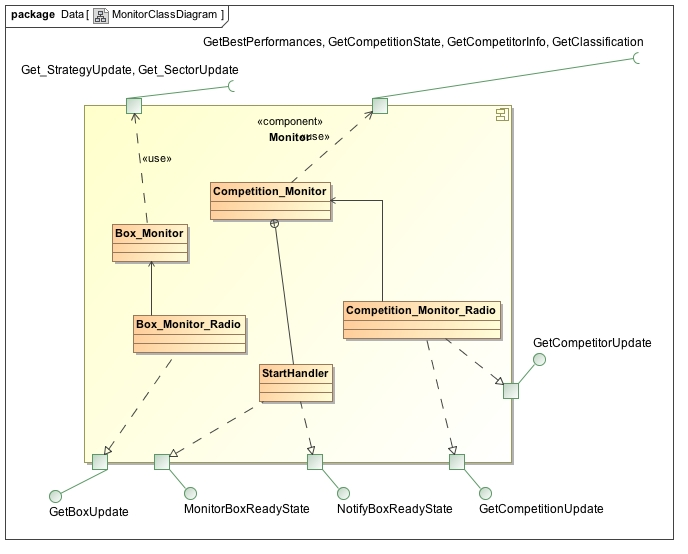
\includegraphics[scale=0.50]{img/ClassDiagrams/MonitorClassDiagram.jpg}
\caption{Class diagram - Monitor}
\end{figure}
\end{center}
\emph{Monitor} si suddivide in due sotto-componenti: \textbf{Box\_Monitor} e \textbf{Competition\_Monitor}. La prima \`{e} dedicata alle informazioni
esposte dal \emph{Box}, l'altra a quelle esposte dalla \emph{Competition}.\\
\textbf{Box\_Monitor} produce i dati interrogando la componente \emph{Box}, precisamente \textbf{Box\_Data}, unit\`{a} che vedremo in seguito,
tramite il metodo \underline{Get\_Info}, grazie al quale si ottiene un oggetto che contiene le informazioni inerenti all'ultimo settore
completato dal concorrente (comprese le medie di consumo) e, se disponibile, la strategia calcolata dal \emph{Box} per la lap successiva.\\\\
\textbf{Competition\_Monitor} si appoggia a \emph{Stats} per reperire le informazioni richieste. I metodi che espone sono:
\begin{description}
\item{\textbf{procedure Get\_CompetitionInfo( TimeInstant : FLOAT; ClassificationTimes : out Common.FLOAT\_ARRAY\_POINT; XMLInfo : out Unbounded\_String.Unbounded\_String);}}\\
la procedura inizializza la stringa con le informazioni di competizione in formato XML. Tali informazioni riguardano il posizionamento
dei concorrenti all'istante dato (quale tratto stanno percorrendo e in che lap), le migliori performance fino all'istante dato e la classifica
aggiornata all'ultima lap in corso, con tempi e concorrenti doppiati. Il metodo si appoggia ai metodi forniti da \textbf{Competition\_Stats}
per reperire le informazioni necessarie.
\item{\textbf{procedure Get\_CompetitorInfo(lap : INTEGER; sector : INTEGER ; id : INTEGER; time : out FLOAT; updString : out Unbounded\_String.Unbounded\_String);}}\\
la procedura fornisce le informazioni di un concorrente aggiornate al settore e lap richieste. Il metodo si appoggia a \textbf{OnBoardComputer}
per reperire le informazioni date, precisamente utilizzando il metodo \underline{Get\_BoxInfo} utilizzando come parametro un riferimento
al \textbf{Computer} del concorrente di cui si richiedono le informazioni.
\end{description}
Queste classi non comunicano direttamente con i loro clienti, ma comunicano tramite un intermediario: \textbf{Box\_Monitor\_Radio} e 
\textbf{Competition\_Monitor\_Radio}, ai quali viene demandato il compito di gestire le comunicazione distribuita tramite Polyorb (usando
il protocollo CORBA).
\newpage
\subsubsection{Box}
\label{box_class}
\begin{center}
\begin{figure}[h!]
\advance\leftskip-1.3cm
	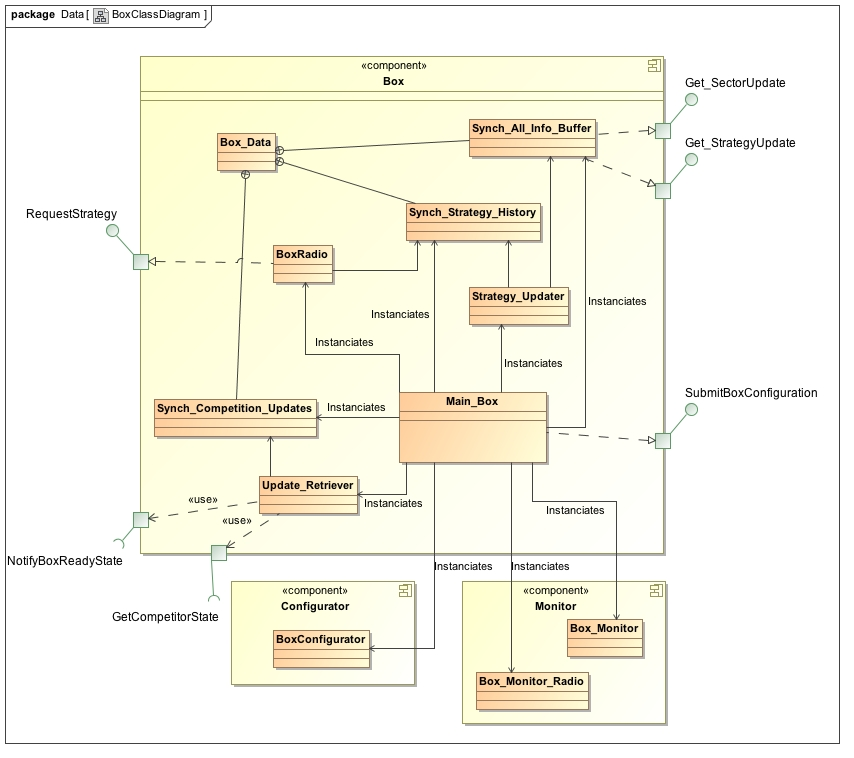
\includegraphics[scale=0.50]{img/ClassDiagrams/BoxClassDiagram.jpg}
\caption{Class diagram - Box}
\end{figure}
\end{center}
Il \emph{Box} \`{e} una componente che si occupa di assistere la gara del concorrete. A tale scopo sono stati previsti due task con le seguenti 
caratteristiche:
\begin{description}
\item{\textbf{Update\_Retriever}}:\\
Come il nome suggerisce, questa unit\`{a} \`{e} finalizzata a recuperare gli aggiornamenti di gara relativi al concorrente associato al box.
A tale scopo, il task si connette al \textbf{Competition\_Monitor} per ottenere un pacchetto di informazioni aggiornato alla fine di ogni 
settore. Tali informazioni vengono convertite in un formato compatibile con il sistema (vengono ricevute in XML e convertite in un oggetto
\textbf{Competition\_Update}). Fatto ci\`{o}, gli aggiornamenti vengono inseriti nel buffer \textbf{Synch\_Competition\_Updates}. Il task
\textbf{Strategy\_Updater} potr\`{a} cos\`{i} leggere gli aggiornamenti non appena disponibili (essendo tale buffer condiviso fra i due task).\\
Il task richiede le informazioni per lap e settore. Se un'informazione non \`{e} ancora stata prodotta, il thread verr\`{a} messo in attesa.
\item{\textbf{Strategy\_Updated}}:\\
L'entit\`{a} rappresenta una parte dell'``intelligenza artificiale'' del sistema. Raccoglie gli aggiornamenti di gara dal buffer \textbf{Synch\_Competition\_Updates}
man mano che essi vengono aggiunti. Tali aggiornamenti vengono di volta in volta usati per aggiornare le medie sui consumi
e aggiornare la strategia di gara. L'aggiornamento della strategia avviene alla fine di ogni secondo settore.
Una volta ottenuto l'aggiornamento del secondo settore, vengono usate le informazioni relative al 3$^{\circ}$ settore del giro precedente e quelle
relative al 1$^{\circ}$ e 2$^{\circ}$ settore del giro corrente per computare una nuova strategia. Una volta che la strategia \`{e} stata calcolata
viene inserita nel buffer \textbf{Strategy\_History}, da dove diventa disponibile nel caso il concorrente la richieda.
\end{description}
A supportare la comunicazione dei dati fra entit\`{a} attive vi sono 3 risorse protette contenute nel package \textbf{Box\_Data}:
\begin{description}
\item{\textbf{Synch\_Competition\_Updates}}:\\
Supporta la comunicazione fra \textbf{Update\_Retriever} e \textbf{Strategy\_History}. Contiene le informazioni di settore del 
concorrente raccolte dal task \textbf{Update\_Retriever}. \textbf{Strategy\_History} reperisce le informazioni in ordine
di inserimento.
\item{\textbf{Synch\_Strategy\_History}}:\\
Supporta la comunicazione fra \textbf{Strategy\_History} e \textbf{BoxRadio}. Il primo aggiunge una nuova strategia alla fine di ogni secondo settore
al buffer. Il secondo \`{e} un tramite fra \emph{Competitor} e \emph{Box} e permette al \textbf{TaskCompetitor} di richiedere una strategia
nuova alla fine di ogni lap tramite il metodo \underline{Get\_Strategy}. Se la strategia \`{e} presente, verr\`{a} tornata. 
Altrimenti il thread che si occupa di gestire la richiesta
viene messo in attesa.
\item{\textbf{Synch\_All\_Info\_Buffer}}:\\
Supporta la comunicazione fra \emph{Box} e \textbf{Box\_Monitor}.Questa risorse \`{e} destinata a contenere tutte le informazioni legate ai box.
Oltre alle informazioni grezze di settore sul concorrente, la risorsa colleziona anche le medie calcolate
dai box e le strategie ogni qualvolta ne siano disponibili di nuove. Le informazioni sono ordinate cronologicamente e associate
ad un indice. L'indice va da 1 a $3 * Lap Totali$, poich\`{e} i settori sono tre. Se un'informazione relativa ad un settore e ad una lap non
\`{e} disponibile, il richiedente viene messo in attesa fino a che l'aggiornamento non risulti disponibile.
\end{description}
Si pu\`{o} constatare che a concorrere per le informazioni collezionate nel \emph{Box} non vi sono solo unit\`{a} interne alla componente, ma anche
thread che agiscono da altre componenti. Tali thread sono il \textbf{TaskCompetitor} lato \emph{Competition} e l'interfaccia di visualizzazione
delle informazioni del box lato \emph{Screen}. Il primo richiede una nuova strategia alla fine di ogni lap tramite \textbf{CompetitorRadio} (lato
\emph{Competition}) che si mette in contatto con \textbf{BoxRadio} che comunica direttamente con \textbf{Synch\_Strategy\_History} per recuperare
la strategia richiesta o essere messo in attesa.\\
Il secondo (\emph{Screen}) richiede tutte le informazioni dall'indice 1 all'indice massimo contenute in \textbf{Synch\_All\_Info\_Buffer} tramite
la parte del \emph{Monitor} destinata ai box. Le informazioni tornate possono riguardare solo un aggiornamento di settore o anche di strategia,
in base a quanto disponibile per quell'indice.\\
\\
Infine il \textbf{Main\_Box} \`{e} destinato ad inizializzare e configurare le risorse protette condivise e i task e istanziare gli oggetti ORB necessari 
alla comunicazione fra componenti.
\newpage
\subsubsection{Configurator}
\begin{center}
\begin{figure}[h!]
	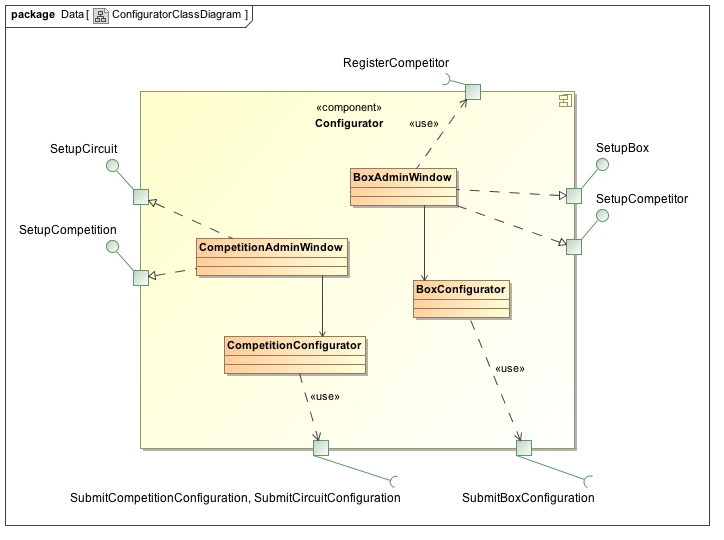
\includegraphics[scale=0.50]{img/ClassDiagrams/ConfiguratorClassDiagram.jpg}
\caption{Class diagram - Configurator}
\end{figure}
\end{center}
La componente, come gi\`{a} accennato, gestisce la configurazione delle componenti \emph{Box} e \emph{Competition}. Pu\`{o} essere vista come suddivisa
a sua volta in due ulteriori sotto-componenti, una destinata all'inserimento dati e l'altra destinata alla comunicazione dei dati alla logica
sottostante. Vediamo infatti nel diagramma due classi \textbf{CompetitionAdminWindow} e \textbf{BoxAdminWindow} che offrono all'utente
un'interfaccia di configurazione (scritta in Java) per \emph{Competition} e \emph{Box}; queste due classi sono legate ai rispettivi ``configurator'',
ovvero classi che permettono l'intercomunicazione fra linguaggi diversi, di modo quindi che i dati inseriti nelle interfacce utente
possano essere trasferiti alle componenti sottostanti per la configurazione e inizializzazione. In dettaglio:
\begin{description}
\item{\textbf{CompetitionConfigurationWindow}}:\\
Utilizzata per impostare i parametri di gara, ovvero:
\begin{itemize}
\item numero lap
\item numero concorrenti
\item file da cui leggere il circuito
\end{itemize}
Una volta impostati i parametri essi verranno sottomessi via \textbf{CompetitionConfigurator} alla \emph{Competition} per la
configurazione e l'inizializzazione.
\item{\textbf{BoxConfigurationWindow}}:\\
Utilizzata per impostare le caratteristiche statiche del concorrente associato al box 
(fare riferimento al capitolo \ref{competitor} per informazioni su tali parametri), dettagli riguardanti il box stesso, ovvero la strategia 
(fare riferimento al capitolo \ref{box} per ulteriori dettagli) e la configurazione iniziale dell'auto, ovvero tipo di gomme e quantit\`{a} di
benzina iniziale. Queste informazioni vengono poi utilizzate per registrare il concorrente alla competizione (tramite il \textbf{RegistrationHandler}
della componente \emph{Competition}). Una volta registrato il concorrente si potranno ottenere il resto delle informazioni necessarie
ad inizializzare il box, ovvero numero di giri e lunghezza circuito (per esempio). \`{E} quindi ora possibile inviare i parametri di configurazione
al \emph{Box} tramite il \textbf{BoxConfigurator}.
\end{description}
\newpage
\subsubsection{Screen}
\begin{center}
\begin{figure}[h!]
	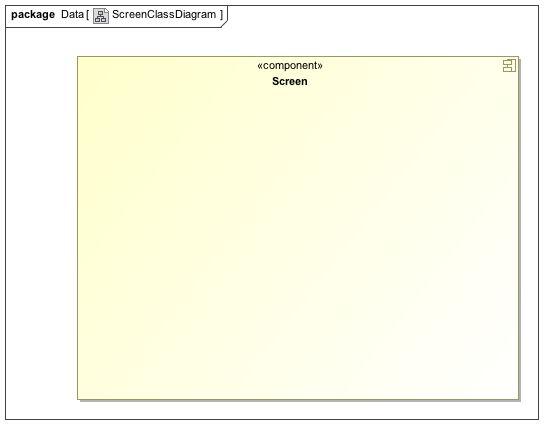
\includegraphics[scale=0.50]{img/ClassDiagrams/ScreenClassDiagram.jpg}
\caption{Class diagram - Screen}
\end{figure}
\begin{description}
\item{\textbf{BoxScreen}}:\\
La classe \textbf{BoxScreen} visualizza l'andamento della competizione da parte del concorrente a cui si riferisce.Questa finestra viene avviata dopo che il concorrente si \`{e} registrato alla competizione. Una volta avviato si mette in ascolto sul \emph{Box\_Monitor\_Radio} che ritorna (quando disponibili) le informazioni relative all'andamento del proprio concorrente, visualizzando tempi, posizione sulla pista, usura delle gomme e livello della benzina.
\item{\textbf{ScreenTv}}:\\
La classe \textbf{ScreenTv} \`{e} l'implementazione dell'interfaccia \textbf{TvPanelInterface} e si occupa di offrire una visualizzazione dei dati di gara.
Quando viene creato lo ScreenTv la connessione con il monitor di sistema \`{e} gi\`{a} stata effettuata ed \`{e} quindi funzionante. Tramite il riferimento al monitor lo ScreenTv \`{e} in grado di ottenere inizialmente le informazioni statiche della gara tramite il metodo \underline{Get\_CompetitionConfiguration} e utilizzarle per costruire la GUI. Successivamente si mette in ascolto sul monitor aspettando l'iscrizione dei concorrenti.Ad iscrizione avvenuta vengono stampate le informazioni relative ai concorrenti. Successivamente, quando parte la gara, lo screenTv comincia ad acquisire informazioni dal monitor. La richiesta viene effettuata ogni intervallo di tempo (fissato per lo screen della competizione, configurabile per lo screen di una tv generica). Ogni volta che viene richiesto un aggiornamento possono presentarsi due situazioni. La prima \`{e} la disponibilit\`{a} delle informazioni che quindi vengono lette e la gui viene cos\`{i} aggiornata con i valori opportuni, la seconda \`{e} la non disponibilit\`{a} di aggiornamenti, in tal caso lo screenTv rimane in attesa.
\end{description}
\end{center}
%Diagrammi delle classi per ogni componente
%"Analisi della concorrenza"
\subsection{Analisi della concorrenza}
	%. analisi dell'interazione risorse e task (senza menzionare la distribuzione)
	  %TaskCompetitor - Synch_Checkpoint
\subsubsection{Interazione Competitor - Circuit}
La strategia adottata per permettere ai concorrenti di percorrere la pista \`{e} stata descritta ad alto livello nel capitolo \ref{strategia_simulazione}.
Tale strategia \`{e} indipendente dal linguaggio o dall'implementazione, quindi il codice scritto ha semplicemente tradotto la teoria in pratica.
Gli aspetti legati all'implementazione a cui si \`{e} dovuto prestare attenzione invece sono descritti di seguito:
\begin{description}
\item{Accesso simultaneo ai checkpoint}\\
Per garantire che il checkpoint sia acceduto in modo mutamente esclusivo fra task, \`{e} stato sufficiente inserirlo in una risorsa protetta:
\textbf{Synch\_Checkpoint}. Tale risorsa offre i metodi necessari ai \textbf{TaskCompetitor} per segnalare il proprio arrivo sulla coda,
``scrivere'' il tempo di arrivo limite ecc. in modo da evitare race condition.
\item{Prima posizione raggiunta}\\
Come si \`{e} visto, quando un concorrente arriva ad un checkpoint deve segnalare il suo arrivo effettivo e, una volta raggiunta la prima posizione
nella coda del checkpoint, iniziare a valutare il path da percorrere. Per mettere in pratica il sistema progettato, \`{e} stato necessario avvalersi
di un'ulteriore risorsa protetta chiamata \textbf{Waiting\_Block}. Ne viene istanziata una lista in ogni \textbf{Synch\_Checkpoint} (una lista
lunga quanto il numero di concorrenti). Ogni elemento della lista \`{e} associato ad un concorrente. 
Quando un concorrente necessita di attendere su una qualunque condizione, viene messo in attesa
sul suo rispettivo \textbf{Waiting\_Block}. Quando la condizione si verifica, il thread che ha causato il cambio
di condizione invoca il metodo \underline{Notify} nel \textbf{Waitin\_Block}, che risveglia il thread che era in attesa.
La condizione per cui viene utilizzata questa struttura \`{e} il raggiungimento della prima posizione nella coda del checkpoint. Il seguente diagramma
descrive la sequenza di eventi che portano il \textbf{TaskCompetitor} da segnalare il suo arrivo al checkpoint all'ottenere i path tra cui
scegliere per effettuare l'attraversamento del tratto.
\begin{center}
\begin{figure}[h!]
\advance\leftskip-2.2cm
	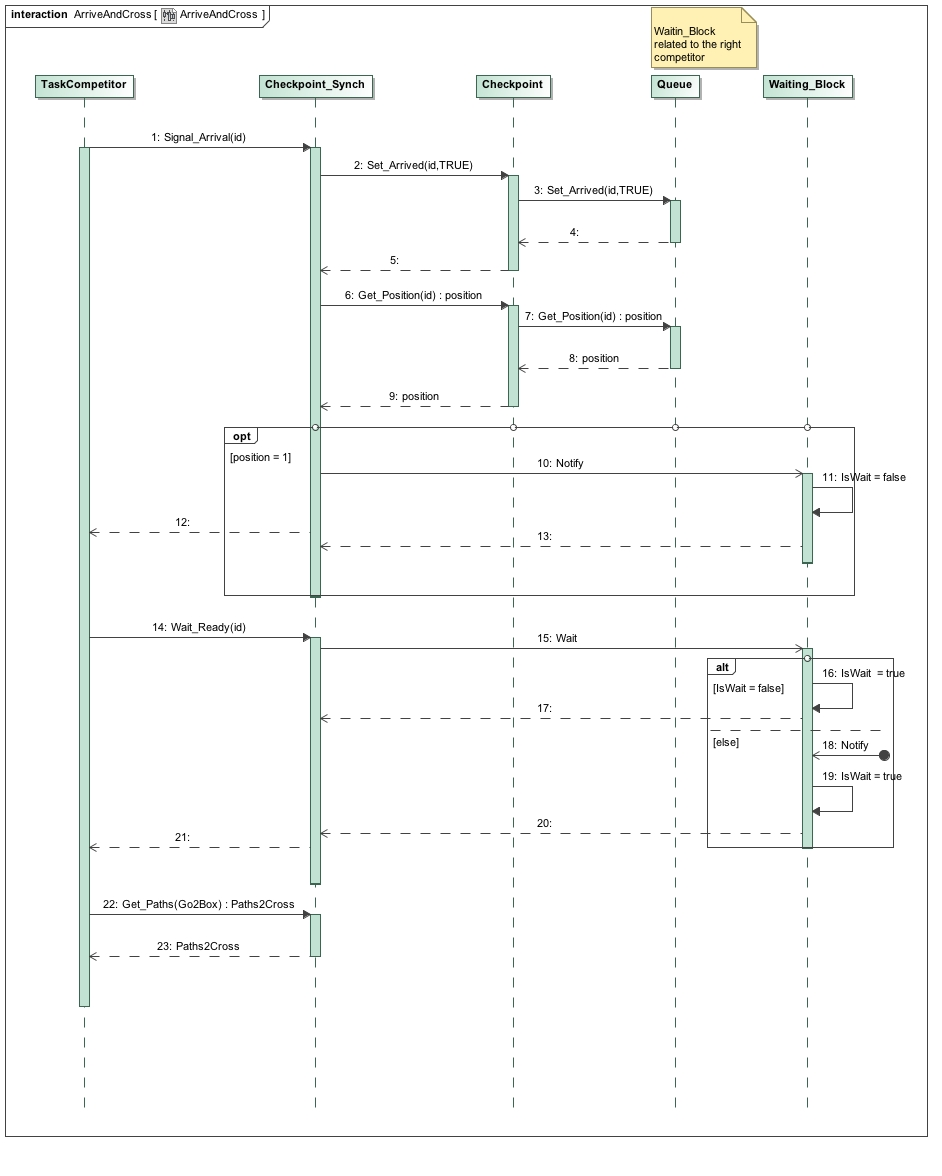
\includegraphics[scale=0.50,height=20cm]{img/SequenceDiagrams/ArriveAndCross.jpg}
\caption{Sequence Diagram - Arrivo al checkpoint e recupero lista traiettorie}
\end{figure}
\end{center}
\clearpage
Prima di passare alla spiegazione del diagramma \`{e} necessario premettere in quali casi un concorrente pu\`{o} cambiare stato nella coda del \textbf{Synch\_Checkpoint}:
\begin{itemize}
\item \textsc{cambio posizione}: pu\`{o} avvenire quando un qualunque concorrente segna un nuovo tempo minimo (o effettivo) 
di arrivo con \underline{Set\_ArrivalTime} o quando un concorrente viene rimosso dal checkpoint con il metodo \underline{Remove\_Competitor};
\item \textsc{da ``in arrivo'' ad ``arrivato'' e viceversa}: avviene su invocazione del metodo \underline{Signal\_Arrival}, quando il concorrente
arriva (passando da ``in arrivo'' ad ``arrivato'') o del metodo \underline{Signal\_Leaving}, quando il concorrente ha finito ed \`{e} pronto
a lasciare il checkpoint (passando da ``arrivato'' a ``in arrivo'').
\end{itemize}
Quando il \textbf{TaskCompetitor} segnala il suo arrivo ( a partire dalla chiamata \textbf{1}), viene segnato l'arrivo effettivo all'interno del checkpoint. Successivamente
viene controllata la posizione del concorrente in coda (chiamate dalla \textbf{6} alla \textbf{9}). Se il concorrente \`{e} primo, \`{e} necessario segnalarlo al rispettivo 
\textbf{Waiting\_Block}, anche se il thread non si \`{e} ancora messo in ``wait'' (giusto per aprire la guardia). Successivamente il thread del \textbf{TaskCompetitor} attende
il suo momento con \underline{Wait\_Ready}. Se era gi\`{a} primo, il metodo ritorna subito, dando la possibilit\`{a} al concorrente di ricevere la lista di path (sicuro che nessun
altro in quel momento la star\`{a} valutando). Altrimenti il thread viene messo in attesa nel \textbf{Waiting\_Block} relativo al concorrente. Il thread viene risvegliato
nel momento in cui un altro \textbf{TaskCompetitor} modifica il suo istante di arrivo limite (facendo in modo che il concorrente in attesa venga a trovarsi nella prima
posizione della coda) o quando viene rimosso dal checkpoint. Eseguendo una qualunque delle azioni accennate nella premessa, il \textbf{TaskCompetitor} verifica quindi
la presenza di un concorrente effettivamente arrivato in prima posizione nella lista ed effettua una \underline{Notify} sul relativo \textbf{Waiting\_Block} (nel diagramma
viene espresso come un evento esterno al punto \textbf{18}). In questo modo il concorrente in attesa pu\`{o} procedere alla valutazione.
\end{description}
\newpage
\subsubsection{Consumatori esterni - Stats}
La sotto-componente \textbf{Competition\_Monitor} espone diverse viste riguardanti i dati relativi alla competizione. Tali dati vengono acceduti in modo ``simultaneo'' 
da qualunque entit\`{a} esterna lo richieda. Viene creato quindi un thread per ogni richiesta proveniente da un nodo distribuito (i \emph{TVScreen} per esempio, di cui
ne potrebbero esistere potenzialmente decine o pi\`{u}). La tecnica adottata
per affrontare il problema ha alla base l'idea che tutte le statistiche vengono calcolate a partire da dati ``grezzi'' relativi ai singoli concorrenti. Essendo ogni
dato riferito ad un istante e ad una specifica posizione nelle competizione (lap numero 2 e checkpoint 5 per esempio), \`{e} possibile calcolare qualunque statistica
che sia riferita ad un istante o ad una posizione (es: i tempi di ogni concorrente alla fine della lap 4).\\
Ad ogni concorrente \`{e} assegnato un array (in \emph{Stats}) in cui ogni posizione \`{e} destinata a contenere un aggiornamento. Gli aggiornamenti sono cronologicamente ordinati.
\`{E} quindi possibile richiedere la posizione del concorrente nel circuito all'istante \emph{t} semplicemente scorrendo l'array. Ogni informazione \`{e} contenuta in una risorsa
protetta la cui lettura viene aperta solo nel momento in cui l'aggiornamento relativo viene inserito. Quindi se viene richiesta un'informazione non ancora presente,
il thread richiedente semplicemente rimarr\`{a} in attesa.\\
Volendo ottenere lo stato di gara all'istante \emph{t} sar\`{a} quindi sufficiente ciclare sui concorrenti chiedendo la loro posizione in tale istante, e quando tutti i concorrenti
avranno aggiunto l'aggiornamento richiesto sar\`{a} possibile avere uno snapshot della gara in tale istante.\\
Per la classifica \`{e} stata aggiunta una struttura dati di supporto finalizzata a venire popolata con i dati di fine lap di ogni concorrente (\textbf{Synch\_Classification\_Table}).
\subsubsection{Risorse a due consumatori}
Ci sono infine numerosi casi in cui una risorsa protetta \`{e} acceduta dai classici consumatore e un produttore. Accesso simultaneo di due risorse attive al massimo dunque.
\`{E} il caso, ad esempio, delle informazioni relative al box, \textbf{Synch\_All\_Info\_Buffer}. Tale risorsa viene valorizzata da \textbf{Strategy\_Updater} e 
letta dallo screen relativo al box (tramite \textbf{Box\_Monitor}). Come visto nella sezione \ref{box_class}, il consumatore accede alla risorsa per indice tramite 
\underline{Get\_Info}. Quindi,
se l'informazione di indice richiesto non \`{e} ancora stata inserita, la sentinella \textsc{Ready} verr\`{a} impostata a \textsc{False} e il thread \textbf{riaccodato} in \underline{Wait}
con la guardia \textsc{Ready=True}. Quando il produttore inserisce una nuova risorsa, verr\`{a} impostato \textsc{Ready} a \textsc{True}, di modo che l'eventuale
thread in attesa possa verificare se l'informazione voluta sia stata inserita. In caso affermativo l'informazione viene ritornata. In caso negativo il thread riesegue
la stessa procedure descritta inizialmente. Chiaramente questa tecnica non potrebbe funzionare con pi\`{u} consumatori, poich\`{e} la guardia potrebbe venire cambiata
pi\`{u} volte ad insaputa di un thread che stia venendo \textbf{riaccodato} da \underline{Get\_Info} a \underline{Wait} (la \textbf{requeue} infatti prevede prerilascio). La
soluzione per\`{o} si presta a risolvere il problema per tutte le situazioni in cui non pi\`{u} di un consumatore e un produttore accedano alla stessa risorsa.
\subsubsection{Conclusioni}
Quanto descritto riguarda i casi pi\`{u} problematici di gestione dell'accesso concorrente a risorse. Il resto dei casi viene trattato con semplici risorse protette
e \textbf{entry} con guardie. Non si presenta quindi il rischio di racecondition. Nemmeno starvation dovrebbe essere possibile, 
a meno che per qualche motivo un thread relativo ad un \textbf{TaskCompetitor}
non si interrompa inaspettatamente, bloccando il processo di aggiornamento delle statistiche e quindi la produzione di snapshot di gara.
%"Distribuzione"
\subsection{Distribuzione}
Nella seguente sezione verranno spiegati dettagli fondamentali riguardanti la distribuzione nel sistema.
	%. Elenco risorse distribuite
	%. Interazione risorse distribuite
	%. Misure di fault tolerance
\subsubsection{Componenti distribuite}%Con motivazione
Si \`{e} deciso di permettere la distribuzione delle seguenti componenti:
\begin{itemize}
\item\textbf{\emph{Box}}:\\
La componente \emph{Box} \`{e} possibile avviarla in un nodo separato rispetto alla competizione. \`{E} necessario infatti fornire il \textbf{corbaloc} della competizione
per poter inizializzare tale componente. La scelta \`{e} stata suggerita da due motivazioni. Una, puramente pratica, riguarda un potenziale problema di sovraccarico 
computazionale. Il \emph{Box} infatti, anche se per ora adotta una \emph{AI} con vincoli abbastanza rilassati, potrebbe richiedere una potenza di calcolo superiore
per effettuare dei calcoli estremamente complessi. Si pensi per esempio se venisse adottato un sistema ad apprendimento automatico o un algoritmo di ricerca della
soluzione ottima ad albero per ogni scelta che il \emph{Box} deve prendere. Avere la possibilit\`{a} di poterlo isolare in una macchina dedicata potrebbe significare
un notevole miglioramento nelle prestazioni.\\
La seconda motivazione invece \`{e} legata alla realt\`{a}: i box normalmente comunicano via radio con i propri piloti. Inserire lo strato di comunicazione remota
fra \emph{Competitor} e \emph{Box} \`{e} sembrato quindi un buon inizio per dare maggiore credibilit\`{a} alla simulazione. I problemi di comunicazione fra le radio
di box e pilota si possono tradurre in problemi di rete fra i due nodi ospitanti \emph{Box} e \emph{Competitor}.
\item\textbf{\emph{TVScreen}}:\\
Le TV da cui poter osservare il procedere della gara possono essere inizializzate ovunque, a patto di essere in possesso del \textbf{corbaloc} del monitor di competizione.
Il fatto che le TV (come nella realt\`{a}) potrebbero essere numerose, \`{e} parso sensato pensarle eseguite in nodi differenti da quello della competizione. Anche in questo
caso per evitare il sovraccarico computazionale della macchina ospitante la competizione. Come per i box, se la TV avviata \`{e} una e a solo output testuale (come quella
presentata nel progetto) il problema non si presenterebbe comunque. Ma volendone avviare molte a volendo magari in un futuro estendere le funzionalit\`{a} del sistema
aggiungendo un overlay grafico pi\`{u} interessante alle TV, tornerebbe molto utile in termini di efficienza poterle eseguire in nodi dedicati.
\end{itemize}
\subsubsection{Interazione fra le componenti distribuite}
Le componenti comunicano la maggior parte dei dati appoggiandosi a protocolli XML. Ogni set di informazioni scambiato fra componenti ha il suo schema dedicato. In questo
modo si pu\`{o} avere un formato di rappresentazione dei dati standard, pi\`{u} facilmente manipolabile con le librerie e le conoscenze disponibili. 
Dati che richiedono una precisione maggiore, ovvero gli istanti temporali espressi in \textsc{Float} (che possono crescere notevolmente all'aumentare del tempo di gara),
vengono trasmessi utilizzando il tipo FLOAT fornito dal linguaggio IDL e, per sequenze di lunghezza non conosciuta a priori, utilizzando il tipo IDL definito come segue
\begin{lstlisting}
typedef sequence<float> float_sequence;
\end{lstlisting}
Tale tipo viene poi manipolato in modo diverso in base al linguaggio utilizzato per la componente, rimanendo comunque entro un buon margine di precisione.
\subsubsection{Misure di fault tolerance}
Cavi di rete danneggiati o router intasati potrebbero provocare il malfunzionamento della comunicazione fra le componenti distribuite. Nel caso di malfunzionamento
della comunicazione fra \textbf{TVScreen} e \emph{Competition}, la competizione non viene compromessa. Nella peggiore delle ipotesi il \textbf{TVScreen} non \`{e} in grado
di ottenere i dati richiesti e ritenter\`{a} in seguito. Nel caso uno o pi\`{u} dei nodi ospitanti i \emph{Box} cada o rimanga isolato, la competizione rischierebbe
di essere compromessa. In prossimit\`{a} del checkpoint prima dei box infatti il concorrente effettua una richiesta remota al \emph{Box} per l'aggiornamento della strategia.
Se tale richiesta produce errore, il concorrente rischierebbe di non poter procedere la gara. Si \`{e} deciso quindi di gestire l'arrivo di dati corrotti o la scomparsa di 
connessione semplicemente facendo mantenere al concorrente la stessa strategia adottata al giro precedente.
% Inizializzazione gara
\subsection{Inizializzazione competizione}
Il seguente diagramma di sequenza spiega come avviene la sequenza di init della competizione, a partire dal main della competizione \textbf{main\_competition.adb}.
\`{E} necessario premettere che l'init vero e proprio non avviene eseguendo il file \textbf{main\_competition.adb}. 
\`{E} stato infatti creato uno script (in bash) che effettua l'avvio di tale main e che successivamente inizializza 
l'interfaccia di configurazione (in java) della competizione.
\begin{center}
\begin{figure}[h!]
\advance\leftskip-3.2cm
	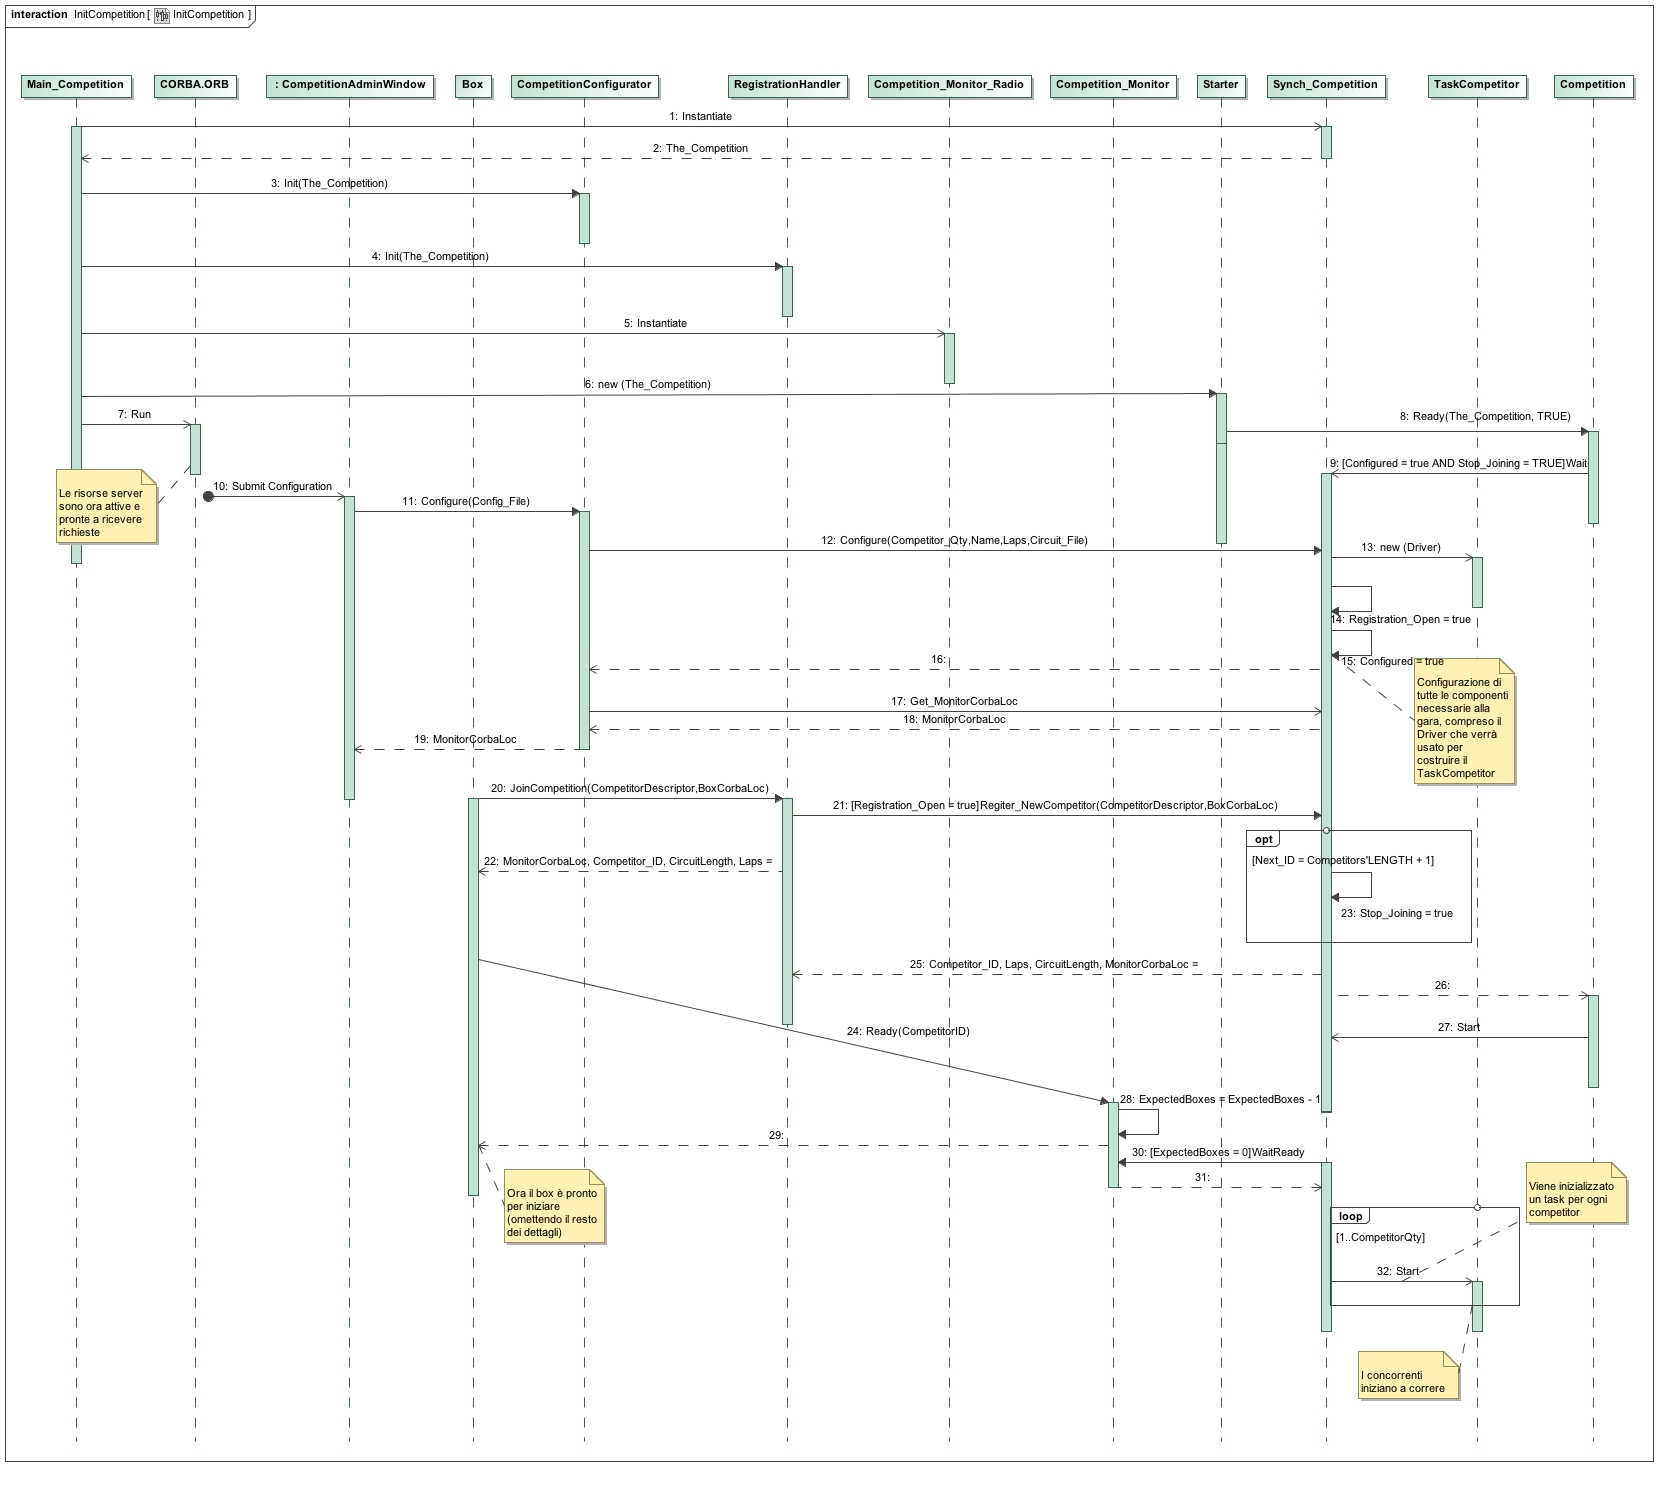
\includegraphics[angle=90,scale=0.35]{img/SequenceDiagrams/InitCompetition.jpg}
\caption{Sequence Diagram - Inizializzazione competizione}
\end{figure}
\end{center}
\clearpage
Una volta avviato il main della competizione, per prima cosa vengono inizializzati tutti i server, vale a dire \textbf{CompetitionConfigurator},
\textbf{RegistrationHandler} \textbf{Competition\_Monitor\_Radio}. Viene avviato un task \textbf{Starter} che rimane in attesa
della configurazione e registrazione concorrenti avvenuti per dare lo \underline{Start} alla gara. Viene inoltre allocato una risorsa protetta di tipo \textbf{Synch\_Competition} pensata
per agevolare la fase di init. Ne viene condivisa un'istanza fra \textbf{CompetitionConfigurator}, \textbf{RegistrationHandler} e \textbf{Starter}.
Tale risorsa permette di regolare i vari step dell'inizializzazione. Finch\`{e} la competizione non viene configurata (dal passo \textbf{10} al passo \textbf{16}),
non sar\`{a} concesso di registrare concorrenti. Una volta configurata la competizione, viene aperta la guardia \textsc{Registration\_Open} e il metodo
\underline{Register\_NewCompetitor} potr\`{a} essere invocato (in \textbf{Synch\_Competition}. L'iscrizione dei concorrenti avviene a partire dai \emph{Box}.
Nel diagramma l'azione iniziale del \emph{Box} e la \textbf{20}. In realt\`{a}, nel nodo del box, viene prima avviato uno script che esegue il main del box
seguito dal main dell'interfaccia (java) di configurazione del concorrente e del box. A configurazione avvenuta, i parametri vengono inviati al server della
competizione invocando il metodo del server \textbf{Registration\_Handler} \underline{Join\_Competition}, come scritto nel diagramma. A iscrizione avvenuta, 
i parametri di configurazione della competizione tornati vengono usati per inizializzare e avviare il box e relativi task grazie a cui successivamente
sar\`{a} possibile mandare il messaggio di \underline{Ready} alla competizione. Per ulteriori dettagli su questa parte, fare riferimento al capitolo
\ref{box_class} relativo al \emph{Box}.\\
Quando tutti i concorrenti sono stati registrati (\textbf{23}), bisogna rimanere in attesa della conferma di avvenuta inizializzazione dei \emph{Box}. Ci\`{o}
avviene quando il thread del task \textbf{Starter} invoca il metodo \underline{Start} del \textbf{Synch\_Competition}, dentro cui viene messo in attesa
sul \textbf{Competition\_Monitor} tramite \underline{Wait\_Ready}. Quando tutti i \emph{Box} hanno dato l'ok, significa che sono pronti per ricevere
richieste dai rispettivi competitor e la gara pu\`{o} cominciare. Vengono cos\`{i} avviati uno ad uno (\textbf{32}) e la competizione ha inizio.
\subsection{Stop competizione}
Lo stop del sistema avviene su 3 livelli: stop dei task, stop delle interfacce utente e stop dei server. Vediamo in dettaglio:
\begin{description}
\item{\textbf{Stop dei task}}:\\
i task che devono essere fermati sono i \textbf{TaskCompetitor} lato competizione e i task \textbf{Update\_Retriever} e \textbf{Strategy\_Updater} lato box.
I primi si fermano in automatico quando le condizioni dell'auto non permettono di procedere (benzina finita o gomme troppo usurate) oppure a competizione finita
(fine ultima lap). I secondi due si fermano quando l'aggiornamento fornito dal monitor della competizione segnala uno stato dell'auto a causa di cui il 
concorrente non pu\`{o} procedere (poca benzina o molta usura gomme), oppure quando il concorrente finisce l'ultima lap (sempre grazie agli aggiornamenti);
\item{\textbf{Stop delle interfacce utente}}:\\
\`{e} sufficiente chiudere le interfacce con il tasto \textbf{x} in alto a destra;
\item{\textbf{Stop dei server}}:\\
una volta finita la gara e chiuse le interfacce utente, \`{e} sufficiente digitare ``q+INVIO'' nelle console dove si sono avviati i main per lanciare un
segnale di terminazione ai programmi (e conseguentemente alle risorse server).
\end{description}
